%&preformat-disser
\RequirePackage[l2tabu,orthodox]{nag} % Раскомментировав, можно в логе получать рекомендации относительно правильного использования пакетов и предупреждения об устаревших и нерекомендуемых пакетах
% Формат А4, 14pt (ГОСТ Р 7.0.11-2011, 5.3.6)
\documentclass[a4paper,14pt,oneside,openany]{memoir}

%% Режим черновика
\makeatletter
\@ifundefined{c@draft}{
  \newcounter{draft}
  \setcounter{draft}{1}  % 0 --- чистовик (максимальное соблюдение ГОСТ)
                         % 1 --- черновик (отклонения от ГОСТ, но быстрая сборка итоговых PDF)
}{}
\makeatother

%% Библиография

%% Внимание! При использовании bibtex8 необходимо удалить все
%% цитирования из  ../common/characteristic.tex
\newcounter{bibliosel}
\setcounter{bibliosel}{1}           % 0 --- встроенная реализация с загрузкой файла через движок bibtex8; 1 --- реализация пакетом biblatex через движок biber
               % общие настройки шаблона
%%% Проверка используемого TeX-движка %%%
\usepackage{iftex}[2013/04/04]
\newif\ifxetexorluatex   % определяем новый условный оператор (http://tex.stackexchange.com/a/47579/79756)
\ifXeTeX
    \xetexorluatextrue
\else
    \ifLuaTeX
        \xetexorluatextrue
    \else
        \xetexorluatexfalse
    \fi
\fi

\RequirePackage{etoolbox}[2015/08/02]               % Для продвинутой проверки разных условий

%%% Поля и разметка страницы %%%
\usepackage{pdflscape}                              % Для включения альбомных страниц
\usepackage{geometry}                               % Для последующего задания полей

%%% Математические пакеты %%%
\usepackage{amsthm,amsfonts,amsmath,amssymb,amscd}  % Математические дополнения от AMS
\usepackage{mathtools}                              % Добавляет окружение multlined

%%%% Установки для размера шрифта 14 pt %%%%
%% Формирование переменных и констант для сравнения (один раз для всех подключаемых файлов)%%
%% должно располагаться до вызова пакета fontspec или polyglossia, потому что они сбивают его работу
\newlength{\curtextsize}
\newlength{\bigtextsize}
\setlength{\bigtextsize}{13.9pt}

\makeatletter
%\show\f@size                                       % неплохо для отслеживания, но вызывает стопорение процесса, если документ компилируется без команды  -interaction=nonstopmode 
\setlength{\curtextsize}{\f@size pt}
\makeatother

%%% Кодировки и шрифты %%%
\ifxetexorluatex
    \usepackage{polyglossia}[2014/05/21]            % Поддержка многоязычности (fontspec подгружается автоматически)
\else
    \RequirePDFTeX                                  % tests for PDFTEX use and throws an error if a different engine is being used
   %%% Решение проблемы копирования текста в буфер кракозябрами
%    \input glyphtounicode.tex
%    \input glyphtounicode-cmr.tex %from pdfx package
%    \pdfgentounicode=1
    \usepackage{cmap}                               % Улучшенный поиск русских слов в полученном pdf-файле
    \defaulthyphenchar=127                          % Если стоит до fontenc, то переносы не впишутся в выделяемый текст при копировании его в буфер обмена
    \usepackage[T2A]{fontenc}                       % Поддержка русских букв
    \usepackage[utf8]{inputenc}[2014/04/30]         % Кодировка utf8
    \usepackage[english, russian]{babel}[2014/03/24]% Языки: русский, английский
    \IfFileExists{pscyr.sty}{\usepackage{pscyr}}{}  % Красивые русские шрифты
\fi

%%% Оформление абзацев %%%
\usepackage{indentfirst}                            % Красная строка

%%% Цвета %%%
\usepackage[dvipsnames,usenames]{color}
\usepackage{colortbl}
%\usepackage[dvipsnames, table, hyperref, cmyk]{xcolor} % Вероятно, более новый вариант, вместо предыдущих двух строк. Конвертация всех цветов в cmyk заложена как удовлетворение возможного требования типографий. Возможно конвертирование и в rgb.

%%% Таблицы %%%
\usepackage{longtable}                              % Длинные таблицы
\usepackage{multirow,makecell}                      % Улучшенное форматирование таблиц

%%% Общее форматирование
\usepackage{soulutf8}                               % Поддержка переносоустойчивых подчёркиваний и зачёркиваний
\usepackage{icomma}                                 % Запятая в десятичных дробях


%%% Гиперссылки %%%
\usepackage[unicode]{hyperref}[2012/11/06]

%%% Изображения %%%
\usepackage{graphicx}[2014/04/25]                   % Подключаем пакет работы с графикой

%%% Списки %%%
\usepackage{enumitem}

%%% Подписи %%%
\usepackage{caption}[2013/05/02]                    % Для управления подписями (рисунков и таблиц) % Может управлять номерами рисунков и таблиц с caption %Иногда может управлять заголовками в списках рисунков и таблиц
\usepackage{subcaption}[2013/02/03]                 % Работа с подрисунками и подобным

%%% Счётчики %%%
\usepackage[figure,table]{totalcount}               % Счётчик рисунков и таблиц
\usepackage{totcount}                               % Пакет создания счётчиков на основе последнего номера подсчитываемого элемента (может требовать дважды компилировать документ)
\usepackage{totpages}                               % Счётчик страниц, совместимый с hyperref (ссылается на номер последней страницы). Желательно ставить последним пакетом в преамбуле

%%% Продвинутое управление групповыми ссылками (пока только формулами) %%%
\ifxetexorluatex
    \usepackage{cleveref}                           % cleveref корректно считывает язык из настроек polyglossia
\else
    \usepackage[russian]{cleveref}                  % cleveref имеет сложности со считыванием языка из babel. Такое решение русификации вывода выбрано вместо определения в documentclass из опасности что-то лишнее передать во все остальные пакеты, включая библиографию.
\fi
\creflabelformat{equation}{#2#1#3}                  % Формат по умолчанию ставил круглые скобки вокруг каждого номера ссылки, теперь просто номера ссылок без какого-либо дополнительного оформления


\ifnumequal{\value{draft}}{1}{% Черновик
    \usepackage[firstpage]{draftwatermark}
    \SetWatermarkText{DRAFT}
    \SetWatermarkFontSize{14pt}
    \SetWatermarkScale{15}
    \SetWatermarkAngle{45}
}{}

  % Пакеты общие для диссертации и автореферата
%%% Прикладные пакеты %%% 
%\usepackage{calc}               % Пакет для расчётов параметров, например длины

%%% Для добавления Стр. над номерами страниц в оглавлении
%%% http://tex.stackexchange.com/a/306950
\usepackage{afterpage}


% Блок схемы

\usepackage{tikz}
\usetikzlibrary{shapes, arrows, chains}
\pgfkeys{/tikz/.cd,% to set the path
	a/.initial=20mm, % initial value
	a/.get=\a, % to get the value from a macro
	a/.store in=\a, % to store the value into a macro
}
\tikzstyle{block} = [
	rectangle,
	aspect = 1.5,
	draw=black,
	align=center,
	text width = 1.5*\a,
	minimum height = \a,
	minimum width = 1.5*\a,]
\tikzstyle{start_stop} = [
	rectangle,
	aspect = 1.5,
	rounded corners=0.25*\a,
	draw=black,
	align=center,
	text width = 1.5*\a,
	minimum height = 0.5*\a,
	minimum width = 1.5*\a,]
\tikzstyle{if} = [
	diamond,
	aspect = 1.5,
	draw=black,
	align=center,
	text width = 1*\a,
	minimum height = 0.5*\a,
	minimum width = 1.5*\a,]	         % Пакеты для диссертации
\usepackage{tabu, tabulary}  %таблицы с автоматически подбирающейся шириной столбцов
\usepackage{fr-longtable}    %ради \endlasthead

\usepackage{svg} % формат векторной графики
% Листинги с исходным кодом программ
\usepackage{fancyvrb}
\usepackage{listings}
\lccode`\~=0\relax %Без этого хака из-за особенностей пакета listings перестают работать конструкции с \MakeLowercase и т. п. в (xe|lua)latex

% Русская традиция начертания греческих букв
\usepackage{upgreek} % прямые греческие ради русской традиции

% Микротипографика
%\ifnumequal{\value{draft}}{0}{% Только если у нас режим чистовика
%    \usepackage[final]{microtype}[2016/05/14] % улучшает представление букв и слов в строках, может помочь при наличии отдельно висящих слов
%}{}

% Отметка о версии черновика на каждой странице
% Чтобы работало надо в своей локальной копии по инструкции
% https://www.ctan.org/pkg/gitinfo2 создать небходимые файлы в папке
% ./git/hooks
% If you’re familiar with tweaking git, you can probably work it out for
% yourself. If not, I suggest you follow these steps:
% 1. First, you need a git repository and working tree. For this example,
% let’s suppose that the root of the working tree is in ~/compsci
% 2. Copy the file post-xxx-sample.txt (which is in the same folder of
% your TEX distribution as this pdf) into the git hooks directory in your
% working copy. In our example case, you should end up with a file called
% ~/compsci/.git/hooks/post-checkout
% 3. If you’re using a unix-like system, don’t forget to make the file executable.
% Just how you do this is outside the scope of this manual, but one
% possible way is with commands such as this:
% chmod g+x post-checkout.
% 4. Test your setup with “git checkout master” (or another suitable branch
% name). This should generate copies of gitHeadInfo.gin in the directories
% you intended.
% 5. Now make two more copies of this file in the same directory (hooks),
% calling them post-commit and post-merge, and you’re done. As before,
% users of unix-like systems should ensure these files are marked as
% executable.
\ifnumequal{\value{draft}}{1}{% Черновик
   \IfFileExists{.git/gitHeadInfo.gin}{                                        
      \usepackage[mark,pcount]{gitinfo2}
      \renewcommand{\gitMark}{rev.\gitAbbrevHash\quad\gitCommitterEmail\quad\gitAuthorIsoDate}
      \renewcommand{\gitMarkFormat}{\color{Gray}\small\bfseries}
   }{}
}{}        % Пакеты для специфических пользовательских задач

%%%%%%%%%%%%%%%%%%%%%%%%%%%%%%%%%%%%%%%%%%%%%%%%%%%%%%
%%%% Файл упрощённых настроек шаблона диссертации %%%%
%%%%%%%%%%%%%%%%%%%%%%%%%%%%%%%%%%%%%%%%%%%%%%%%%%%%%%

%%% Инициализирование переменных, не трогать!  %%%
\newcounter{intvl}
\newcounter{otstup}
\newcounter{contnumeq}
\newcounter{contnumfig}
\newcounter{contnumtab}
\newcounter{pgnum}
\newcounter{chapstyle}
\newcounter{headingdelim}
\newcounter{headingalign}
\newcounter{headingsize}
\newcounter{tabcap}
\newcounter{tablaba}
\newcounter{tabtita}
%%%%%%%%%%%%%%%%%%%%%%%%%%%%%%%%%%%%%%%%%%%%%%%%%%

%%% Область упрощённого управления оформлением %%%

%% Интервал между заголовками и между заголовком и текстом
% Заголовки отделяют от текста сверху и снизу тремя интервалами (ГОСТ Р 7.0.11-2011, 5.3.5)
\setcounter{intvl}{1}               % Коэффициент кратности к размеру шрифта

%% Отступы у заголовков в тексте
\setcounter{otstup}{0}              % 0 --- без отступа; 1 --- абзацный отступ

%% Нумерация формул, таблиц и рисунков
\setcounter{contnumeq}{0}           % Нумерация формул: 0 --- пораздельно (во введении подряд, без номера раздела); 1 --- сквозная нумерация по всей диссертации
\setcounter{contnumfig}{0}          % Нумерация рисунков: 0 --- пораздельно (во введении подряд, без номера раздела); 1 --- сквозная нумерация по всей диссертации
\setcounter{contnumtab}{1}          % Нумерация таблиц: 0 --- пораздельно (во введении подряд, без номера раздела); 1 --- сквозная нумерация по всей диссертации

%% Оглавление
\setcounter{pgnum}{1}               % 0 --- номера страниц никак не обозначены; 1 --- Стр. над номерами страниц (дважды компилировать после изменения)
\settocdepth{subsection}            % до какого уровня подразделов выносить в оглавление
\setsecnumdepth{subsection}         % до какого уровня нумеровать подразделы


%% Текст и форматирование заголовков
\setcounter{chapstyle}{1}           % 0 --- разделы только под номером; 1 --- разделы с названием "Глава" перед номером
\setcounter{headingdelim}{1}        % 0 --- номер отделен пропуском в 1em или \quad; 1 --- номера разделов и приложений отделены точкой с пробелом, подразделы пропуском без точки; 2 --- номера разделов, подразделов и приложений отделены точкой с пробелом.

%% Выравнивание заголовков в тексте
\setcounter{headingalign}{1}        % 0 --- по центру; 1 --- по левому краю

%% Размеры заголовков в тексте
\setcounter{headingsize}{0}         % 0 --- по ГОСТ, все всегда 14 пт; 1 --- пропорционально изменяющийся размер в зависимости от базового шрифта

%% Подпись таблиц
\setcounter{tabcap}{0}              % 0 --- по ГОСТ, номер таблицы и название разделены тире, выровнены по левому краю, при необходимости на нескольких строках; 1 --- подпись таблицы не по ГОСТ, на двух и более строках, дальнейшие настройки: 
%Выравнивание первой строки, с подписью и номером
\setcounter{tablaba}{2}             % 0 --- по левому краю; 1 --- по центру; 2 --- по правому краю
%Выравнивание строк с самим названием таблицы
\setcounter{tabtita}{1}             % 0 --- по левому краю; 1 --- по центру; 2 --- по правому краю
%Разделитель записи «Таблица #» и названия таблицы
\newcommand{\tablabelsep}{space}   % space = пробел, period = точка (определены в подключенных пакетах)

%% Подпись рисунков
%Разделитель записи «Рисунок #» и названия рисунка
\newcommand{\figlabelsep}{emdash}   % emdash = тире, определён в common/styles; period = точка определён в подключенных пакетах

%%% Цвета гиперссылок %%%
% Latex color definitions: http://latexcolor.com/
\definecolor{linkcolor}{rgb}{0,0.6,0}
\definecolor{citecolor}{rgb}{0,0.6,0}
\definecolor{urlcolor}{rgb}{0,0,1}
%\definecolor{linkcolor}{rgb}{0,0,0} %black
%\definecolor{citecolor}{rgb}{0,0,0} %black
%\definecolor{urlcolor}{rgb}{0,0,0} %black               % Упрощённые настройки шаблона

\input{Dissertation/preamblenames}       % Переопределение именований, чтобы можно было и в преамбуле использовать
% Новые переменные, которые могут использоваться во всём проекте
% ГОСТ 7.0.11-2011
% 9.2 Оформление текста автореферата диссертации
% 9.2.1 Общая характеристика работы включает в себя следующие основные структурные
% элементы:
% актуальность темы исследования;
\newcommand{\actualityTXT}{Актуальность темы.}
% степень ее разработанности;
\newcommand{\progressTXT}{Степень разработанности темы.}
% цели и задачи;
\newcommand{\aimTXT}{Целью}
\newcommand{\tasksTXT}{задачи}
% научную новизну;
\newcommand{\noveltyTXT}{Научная новизна:}
% теоретическую и практическую значимость работы;
%\newcommand{\influenceTXT}{Теоретическая и практическая значимость}
% или чаще используют просто
\newcommand{\influenceTXT}{Практическая значимость.}
% методологию и методы исследования;
\newcommand{\methodsTXT}{Mетодология и методы исследования.}
% положения, выносимые на защиту;
\newcommand{\defpositionsTXT}{Основные положения, выносимые на~защиту:}
% степень достоверности и апробацию результатов.
\newcommand{\reliabilityTXT}{Достоверность}
\newcommand{\probationTXT}{Апробация работы.}

\newcommand{\contributionTXT}{Личный вклад.}
\newcommand{\publicationsTXT}{Публикации.}


\newcommand{\authorbibtitle}{Публикации автора по теме диссертации}
\newcommand{\vakbibtitle}{В изданиях из списка ВАК РФ}
\newcommand{\notvakbibtitle}{В прочих изданиях}
\newcommand{\confbibtitle}{В сборниках трудов конференций}
\newcommand{\fullbibtitle}{Список литературы} % (ГОСТ Р 7.0.11-2011, 4)
  % Новые переменные, которые могут использоваться во всём проекте

% !TeX spellcheck = de_DE
%%% Основные сведения %%%
\newcommand{\thesisAuthor}             % Диссертация, ФИО автора
{%
    \texorpdfstring{% \texorpdfstring takes two arguments and uses the first for (La)TeX and the second for pdf
        Сатышев Антон Сергеевич% так будет отображаться на титульном листе или в тексте, где будет использоваться переменная
    }{%
        Сатышев, Антон Сергеевич% эта запись для свойств pdf-файла. В таком виде, если pdf будет обработан программами для сбора библиографических сведений, будет правильно представлена фамилия.
    }%
}
\newcommand{\thesisAuthorShort}        % Диссертация, ФИО автора инициалами
{\todo{А.С.~Сатышев}}

\newcommand{\thesisUdk}                % Диссертация, УДК
{\todo{xxx.xxx}}
\newcommand{\thesisTitle}              % Диссертация, название
{\texorpdfstring{\MakeUppercase{Обоснование рационального радиуса закругления рабочей кромки дискового режущего инструмента для разрушения снежно-ледяных образований}}{Обоснование рационального радиуса закругления рабочей кромки дискового режущего инструмента для разрушения снежно-ледяных образований}}
\newcommand{\thesisSpecialtyNumber}    % Диссертация, специальность, номер
{\texorpdfstring{05.11.13}{05.11.13}}
\newcommand{\thesisSpecialtyTitle}     % Диссертация, специальность, название
{\texorpdfstring{Приборы и методы контроля природной среды, веществ, материалов и изделий (технические науки)}{Приборы и методы контроля природной среды, веществ, материалов и изделий (технические науки)}}
\newcommand{\thesisDegree}             % Диссертация, ученая степень
{кандидата технических наук}
\newcommand{\thesisDegreeShort}        % Диссертация, ученая степень, краткая запись
{\todo{канд. тех. наук}}
\newcommand{\thesisCity}               % Диссертация, город написания диссертации
{Красноярск}
\newcommand{\thesisYear}               % Диссертация, год написания диссертации
{2017}
\newcommand{\thesisOrganization}       % Диссертация, организация
{Федеральное государственное автономное образовательное учреждение\protect\\высшего профессионального образования\protect\\<<Сибирский федеральный университет>>}
\newcommand{\thesisOrganizationShort}  % Диссертация, краткое название организации для доклада
{СФУ}

\newcommand{\thesisInOrganization}     % Диссертация, организация в предложном падеже: Работа выполнена в ...
{Сибирском федеральном университет}

\newcommand{\supervisorFio}            % Научный руководитель, ФИО
{Ганжа Владимир Александрович}
\newcommand{\supervisorRegalia}        % Научный руководитель, регалии
{кандидат технических наук, доцент}
\newcommand{\supervisorFioShort}       % Научный руководитель, ФИО
{В.А.~Ганжа}
\newcommand{\supervisorRegaliaShort}   % Научный руководитель, регалии
{к.т.н.,доц.}


\newcommand{\opponentOneFio}           % Оппонент 1, ФИО
{\todo{Фамилия Имя Отчество}}
\newcommand{\opponentOneRegalia}       % Оппонент 1, регалии
{\todo{доктор физико-математических наук, профессор}}
\newcommand{\opponentOneJobPlace}      % Оппонент 1, место работы
{\todo{Не очень длинное название для места работы}}
\newcommand{\opponentOneJobPost}       % Оппонент 1, должность
{\todo{старший научный сотрудник}}

\newcommand{\opponentTwoFio}           % Оппонент 2, ФИО
{\todo{Фамилия Имя Отчество}}
\newcommand{\opponentTwoRegalia}       % Оппонент 2, регалии
{\todo{кандидат физико-математических наук}}
\newcommand{\opponentTwoJobPlace}      % Оппонент 2, место работы
{\todo{Основное место работы c длинным длинным длинным длинным названием}}
\newcommand{\opponentTwoJobPost}       % Оппонент 2, должность
{\todo{старший научный сотрудник}}

\newcommand{\leadingOrganizationTitle} % Ведущая организация, дополнительные строки
{\todo{Федеральное государственное бюджетное образовательное учреждение высшего профессионального образования с~длинным длинным длинным длинным названием}}

\newcommand{\defenseDate}              % Защита, дата
{\todo{DD mmmmmmmm YYYY~г.~в~XX часов}}
\newcommand{\defenseCouncilNumber}     % Защита, номер диссертационного совета
{\todo{Д\,123.456.78}}
\newcommand{\defenseCouncilTitle}      % Защита, учреждение диссертационного совета
{\todo{Название учреждения}}
\newcommand{\defenseCouncilAddress}    % Защита, адрес учреждение диссертационного совета
{\todo{Адрес}}
\newcommand{\defenseCouncilPhone}      % Телефон для справок
{\todo{+7~(0000)~00-00-00}}

\newcommand{\defenseSecretaryFio}      % Секретарь диссертационного совета, ФИО
{\todo{Фамилия Имя Отчество}}
\newcommand{\defenseSecretaryRegalia}  % Секретарь диссертационного совета, регалии
{\todo{д-р~физ.-мат. наук}}            % Для сокращений есть ГОСТы, например: ГОСТ Р 7.0.12-2011 + http://base.garant.ru/179724/#block_30000

\newcommand{\synopsisLibrary}          % Автореферат, название библиотеки
{\todo{Название библиотеки}}
\newcommand{\synopsisDate}             % Автореферат, дата рассылки
{\todo{DD mmmmmmmm YYYY года}}

% To avoid conflict with beamer class use \providecommand
\providecommand{\keywords}%            % Ключевые слова для метаданных PDF диссертации и автореферата
{}      % Основные сведения
\input{common/styles}    % Стили общие для диссертации и автореферата
\input{Dissertation/disstyles}           % Стили для диссертации
% для вертикального центрирования ячеек в tabulary
\def\zz{\ifx\[$\else\aftergroup\zzz\fi}
%$ \] % <-- чиним подсветку синтаксиса в некоторых редакторах
\def\zzz{\setbox0\lastbox
\dimen0\dimexpr\extrarowheight + \ht0-\dp0\relax
\setbox0\hbox{\raise-.5\dimen0\box0}%
\ht0=\dimexpr\ht0+\extrarowheight\relax
\dp0=\dimexpr\dp0+\extrarowheight\relax 
\box0
}



\lstdefinelanguage{Renhanced}%
{keywords={abbreviate,abline,abs,acos,acosh,action,add1,add,%
        aggregate,alias,Alias,alist,all,anova,any,aov,aperm,append,apply,%
        approx,approxfun,apropos,Arg,args,array,arrows,as,asin,asinh,%
        atan,atan2,atanh,attach,attr,attributes,autoload,autoloader,ave,%
        axis,backsolve,barplot,basename,besselI,besselJ,besselK,besselY,%
        beta,binomial,body,box,boxplot,break,browser,bug,builtins,bxp,by,%
        c,C,call,Call,case,cat,category,cbind,ceiling,character,char,%
        charmatch,check,chol,chol2inv,choose,chull,class,close,cm,codes,%
        coef,coefficients,co,col,colnames,colors,colours,commandArgs,%
        comment,complete,complex,conflicts,Conj,contents,contour,%
        contrasts,contr,control,helmert,contrib,convolve,cooks,coords,%
        distance,coplot,cor,cos,cosh,count,fields,cov,covratio,wt,CRAN,%
        create,crossprod,cummax,cummin,cumprod,cumsum,curve,cut,cycle,D,%
        data,dataentry,date,dbeta,dbinom,dcauchy,dchisq,de,debug,%
        debugger,Defunct,default,delay,delete,deltat,demo,de,density,%
        deparse,dependencies,Deprecated,deriv,description,detach,%
        dev2bitmap,dev,cur,deviance,off,prev,,dexp,df,dfbetas,dffits,%
        dgamma,dgeom,dget,dhyper,diag,diff,digamma,dim,dimnames,dir,%
        dirname,dlnorm,dlogis,dnbinom,dnchisq,dnorm,do,dotplot,double,%
        download,dpois,dput,drop,drop1,dsignrank,dt,dummy,dump,dunif,%
        duplicated,dweibull,dwilcox,dyn,edit,eff,effects,eigen,else,%
        emacs,end,environment,env,erase,eval,equal,evalq,example,exists,%
        exit,exp,expand,expression,External,extract,extractAIC,factor,%
        fail,family,fft,file,filled,find,fitted,fivenum,fix,floor,for,%
        For,formals,format,formatC,formula,Fortran,forwardsolve,frame,%
        frequency,ftable,ftable2table,function,gamma,Gamma,gammaCody,%
        gaussian,gc,gcinfo,gctorture,get,getenv,geterrmessage,getOption,%
        getwd,gl,glm,globalenv,gnome,GNOME,graphics,gray,grep,grey,grid,%
        gsub,hasTsp,hat,heat,help,hist,home,hsv,httpclient,I,identify,if,%
        ifelse,Im,image,\%in\%,index,influence,measures,inherits,install,%
        installed,integer,interaction,interactive,Internal,intersect,%
        inverse,invisible,IQR,is,jitter,kappa,kronecker,labels,lapply,%
        layout,lbeta,lchoose,lcm,legend,length,levels,lgamma,library,%
        licence,license,lines,list,lm,load,local,locator,log,log10,log1p,%
        log2,logical,loglin,lower,lowess,ls,lsfit,lsf,ls,machine,Machine,%
        mad,mahalanobis,make,link,margin,match,Math,matlines,mat,matplot,%
        matpoints,matrix,max,mean,median,memory,menu,merge,methods,min,%
        missing,Mod,mode,model,response,mosaicplot,mtext,mvfft,na,nan,%
        names,omit,nargs,nchar,ncol,NCOL,new,next,NextMethod,nextn,%
        nlevels,nlm,noquote,NotYetImplemented,NotYetUsed,nrow,NROW,null,%
        numeric,\%o\%,objects,offset,old,on,Ops,optim,optimise,optimize,%
        options,or,order,ordered,outer,package,packages,page,pairlist,%
        pairs,palette,panel,par,parent,parse,paste,path,pbeta,pbinom,%
        pcauchy,pchisq,pentagamma,persp,pexp,pf,pgamma,pgeom,phyper,pico,%
        pictex,piechart,Platform,plnorm,plogis,plot,pmatch,pmax,pmin,%
        pnbinom,pnchisq,pnorm,points,poisson,poly,polygon,polyroot,pos,%
        postscript,power,ppoints,ppois,predict,preplot,pretty,Primitive,%
        print,prmatrix,proc,prod,profile,proj,prompt,prop,provide,%
        psignrank,ps,pt,ptukey,punif,pweibull,pwilcox,q,qbeta,qbinom,%
        qcauchy,qchisq,qexp,qf,qgamma,qgeom,qhyper,qlnorm,qlogis,qnbinom,%
        qnchisq,qnorm,qpois,qqline,qqnorm,qqplot,qr,Q,qty,qy,qsignrank,%
        qt,qtukey,quantile,quasi,quit,qunif,quote,qweibull,qwilcox,%
        rainbow,range,rank,rbeta,rbind,rbinom,rcauchy,rchisq,Re,read,csv,%
        csv2,fwf,readline,socket,real,Recall,rect,reformulate,regexpr,%
        relevel,remove,rep,repeat,replace,replications,report,require,%
        resid,residuals,restart,return,rev,rexp,rf,rgamma,rgb,rgeom,R,%
        rhyper,rle,rlnorm,rlogis,rm,rnbinom,RNGkind,rnorm,round,row,%
        rownames,rowsum,rpois,rsignrank,rstandard,rstudent,rt,rug,runif,%
        rweibull,rwilcox,sample,sapply,save,scale,scan,scan,screen,sd,se,%
        search,searchpaths,segments,seq,sequence,setdiff,setequal,set,%
        setwd,show,sign,signif,sin,single,sinh,sink,solve,sort,source,%
        spline,splinefun,split,sqrt,stars,start,stat,stem,step,stop,%
        storage,strstrheight,stripplot,strsplit,structure,strwidth,sub,%
        subset,substitute,substr,substring,sum,summary,sunflowerplot,svd,%
        sweep,switch,symbol,symbols,symnum,sys,status,system,t,table,%
        tabulate,tan,tanh,tapply,tempfile,terms,terrain,tetragamma,text,%
        time,title,topo,trace,traceback,transform,tri,trigamma,trunc,try,%
        ts,tsp,typeof,unclass,undebug,undoc,union,unique,uniroot,unix,%
        unlink,unlist,unname,untrace,update,upper,url,UseMethod,var,%
        variable,vector,Version,vi,warning,warnings,weighted,weights,%
        which,while,window,write,\%x\%,x11,X11,xedit,xemacs,xinch,xor,%
        xpdrows,xy,xyinch,yinch,zapsmall,zip},%
    otherkeywords={!,!=,~,$,*,\%,\&,\%/\%,\%*\%,\%\%,<-,<<-},%$
    alsoother={._$},%$
    sensitive,%
    morecomment=[l]\#,%
    morestring=[d]",%
    morestring=[d]'% 2001 Robert Denham
}%

%решаем проблему с кириллицей в комментариях (в pdflatex) https://tex.stackexchange.com/a/103712/79756
\lstset{extendedchars=true,literate={Ö}{{\"O}}1
    {Ä}{{\"A}}1
    {Ü}{{\"U}}1
    {ß}{{\ss}}1
    {ü}{{\"u}}1
    {ä}{{\"a}}1
    {ö}{{\"o}}1
    {~}{{\textasciitilde}}1
    {а}{{\selectfont\char224}}1
    {б}{{\selectfont\char225}}1
    {в}{{\selectfont\char226}}1
    {г}{{\selectfont\char227}}1
    {д}{{\selectfont\char228}}1
    {е}{{\selectfont\char229}}1
    {ё}{{\"e}}1
    {ж}{{\selectfont\char230}}1
    {з}{{\selectfont\char231}}1
    {и}{{\selectfont\char232}}1
    {й}{{\selectfont\char233}}1
    {к}{{\selectfont\char234}}1
    {л}{{\selectfont\char235}}1
    {м}{{\selectfont\char236}}1
    {н}{{\selectfont\char237}}1
    {о}{{\selectfont\char238}}1
    {п}{{\selectfont\char239}}1
    {р}{{\selectfont\char240}}1
    {с}{{\selectfont\char241}}1
    {т}{{\selectfont\char242}}1
    {у}{{\selectfont\char243}}1
    {ф}{{\selectfont\char244}}1
    {х}{{\selectfont\char245}}1
    {ц}{{\selectfont\char246}}1
    {ч}{{\selectfont\char247}}1
    {ш}{{\selectfont\char248}}1
    {щ}{{\selectfont\char249}}1
    {ъ}{{\selectfont\char250}}1
    {ы}{{\selectfont\char251}}1
    {ь}{{\selectfont\char252}}1
    {э}{{\selectfont\char253}}1
    {ю}{{\selectfont\char254}}1
    {я}{{\selectfont\char255}}1
    {А}{{\selectfont\char192}}1
    {Б}{{\selectfont\char193}}1
    {В}{{\selectfont\char194}}1
    {Г}{{\selectfont\char195}}1
    {Д}{{\selectfont\char196}}1
    {Е}{{\selectfont\char197}}1
    {Ё}{{\"E}}1
    {Ж}{{\selectfont\char198}}1
    {З}{{\selectfont\char199}}1
    {И}{{\selectfont\char200}}1
    {Й}{{\selectfont\char201}}1
    {К}{{\selectfont\char202}}1
    {Л}{{\selectfont\char203}}1
    {М}{{\selectfont\char204}}1
    {Н}{{\selectfont\char205}}1
    {О}{{\selectfont\char206}}1
    {П}{{\selectfont\char207}}1
    {Р}{{\selectfont\char208}}1
    {С}{{\selectfont\char209}}1
    {Т}{{\selectfont\char210}}1
    {У}{{\selectfont\char211}}1
    {Ф}{{\selectfont\char212}}1
    {Х}{{\selectfont\char213}}1
    {Ц}{{\selectfont\char214}}1
    {Ч}{{\selectfont\char215}}1
    {Ш}{{\selectfont\char216}}1
    {Щ}{{\selectfont\char217}}1
    {Ъ}{{\selectfont\char218}}1
    {Ы}{{\selectfont\char219}}1
    {Ь}{{\selectfont\char220}}1
    {Э}{{\selectfont\char221}}1
    {Ю}{{\selectfont\char222}}1
    {Я}{{\selectfont\char223}}1
    {і}{{\selectfont\char105}}1
    {ї}{{\selectfont\char168}}1
    {є}{{\selectfont\char185}}1
    {ґ}{{\selectfont\char160}}1
    {І}{{\selectfont\char73}}1
    {Ї}{{\selectfont\char136}}1
    {Є}{{\selectfont\char153}}1
    {Ґ}{{\selectfont\char128}}1
}

% Ширина текста минус ширина надписи 999
\newlength{\twless}
\newlength{\lmarg}
\setlength{\lmarg}{\widthof{999}}   % ширина надписи 999
\setlength{\twless}{\textwidth-\lmarg}


\lstset{ %
%    language=R,                     %  Язык указать здесь, если во всех листингах преимущественно один язык, в результате часть настроек может пойти только для этого языка
    numbers=left,                   % where to put the line-numbers
    numberstyle=\fontsize{12pt}{14pt}\selectfont\color{Gray},  % the style that is used for the line-numbers
    firstnumber=1,                  % в этой и следующей строках задаётся поведение нумерации 5, 10, 15...
    stepnumber=1,                   % the step between two line-numbers. If it's 1, each line will be numbered
    numbersep=5pt,                  % how far the line-numbers are from the code
    backgroundcolor=\color{white},  % choose the background color. You must add \usepackage{color}
    showspaces=false,               % show spaces adding particular underscores
    showstringspaces=false,         % underline spaces within strings
    showtabs=false,                 % show tabs within strings adding particular underscores
    frame=leftline,                 % adds a frame of different types around the code
    rulecolor=\color{black},        % if not set, the frame-color may be changed on line-breaks within not-black text (e.g. commens (green here))
    tabsize=2,                      % sets default tabsize to 2 spaces
    captionpos=t,                   % sets the caption-position to top
    breaklines=true,                % sets automatic line breaking
    breakatwhitespace=false,        % sets if automatic breaks should only happen at whitespace
%    title=\lstname,                 % show the filename of files included with \lstinputlisting;
    % also try caption instead of title
    basicstyle=\fontsize{12pt}{14pt}\selectfont\ttfamily,% the size of the fonts that are used for the code
%    keywordstyle=\color{blue},      % keyword style
    commentstyle=\color{ForestGreen}\emph,% comment style
    stringstyle=\color{Mahogany},   % string literal style
    escapeinside={\%*}{*)},         % if you want to add a comment within your code
    morekeywords={*,...},           % if you want to add more keywords to the set
    inputencoding=utf8,             % кодировка кода
    xleftmargin={\lmarg},           % Чтобы весь код и полоска с номерами строк была смещена влево, так чтобы цифры не вылезали за пределы текста слева
} 

%http://tex.stackexchange.com/questions/26872/smaller-frame-with-listings
% Окружение, чтобы листинг был компактнее обведен рамкой, если она задается, а не на всю ширину текста
\makeatletter
\newenvironment{SmallListing}[1][]
{\lstset{#1}\VerbatimEnvironment\begin{VerbatimOut}{VerbEnv.tmp}}
{\end{VerbatimOut}\settowidth\@tempdima{%
        \lstinputlisting{VerbEnv.tmp}}
    \minipage{\@tempdima}\lstinputlisting{VerbEnv.tmp}\endminipage}    
\makeatother


\DefineVerbatimEnvironment% с шрифтом 12 пт
{Verb}{Verbatim}
{fontsize=\fontsize{12pt}{14pt}\selectfont}

\newfloat[chapter]{ListingEnv}{lol}{Листинг}

\captionsetup[ListingEnv]{
    format=tablecaption,
    labelsep=space,                 % Точка после номера листинга задается значением period
    singlelinecheck=off,
    position=top
}

\captionsetup[lstlisting]{
    format=tablecaption,
    labelsep=space,                 % Точка после номера листинга задается значением period
    singlelinecheck=off,
    position=top
}

\renewcommand{\lstlistingname}{Листинг}

%Общие счётчики окружений листингов
%http://tex.stackexchange.com/questions/145546/how-to-make-figure-and-listing-share-their-counter
% Если смешивать плавающие и не плавающие окружения, то могут быть проблемы с нумерацией
\makeatletter
\AtBeginDocument{%
    \let\c@ListingEnv\c@lstlisting
    \let\theListingEnv\thelstlisting
    \let\ftype@lstlisting\ftype@ListingEnv % give the floats the same precedence
}
\makeatother

% значок С++ — используйте команду \cpp
\newcommand{\cpp}{%
    C\nolinebreak\hspace{-.05em}%
    \raisebox{.2ex}{+}\nolinebreak\hspace{-.10em}%
    \raisebox{.2ex}{+}%
}

%%%  Чересстрочное форматирование таблиц
%% http://tex.stackexchange.com/questions/278362/apply-italic-formatting-to-every-other-row
\newcounter{rowcnt}
\newcommand\altshape{\ifnumodd{\value{rowcnt}}{\color{red}}{\vspace*{-1ex}\itshape}}
% \AtBeginEnvironment{tabular}{\setcounter{rowcnt}{1}}
% \AtEndEnvironment{tabular}{\setcounter{rowcnt}{0}}

%%% Ради примера во второй главе
\let\originalepsilon\epsilon
\let\originalphi\phi
\let\originalkappa\kappa
\let\originalle\le
\let\originalleq\leq
\let\originalge\ge
\let\originalgeq\geq
\let\originalemptyset\emptyset
\let\originaltan\tan
\let\originalcot\cot
\let\originalcsc\csc

%%% Русская традиция начертания математических знаков
\renewcommand{\le}{\ensuremath{\leqslant}}
\renewcommand{\leq}{\ensuremath{\leqslant}}
\renewcommand{\ge}{\ensuremath{\geqslant}}
\renewcommand{\geq}{\ensuremath{\geqslant}}
\renewcommand{\emptyset}{\varnothing}

%%% Русская традиция начертания математических функций (на случай копирования из зарубежных источников)
\renewcommand{\tan}{\operatorname{tg}}
\renewcommand{\cot}{\operatorname{ctg}}
\renewcommand{\csc}{\operatorname{cosec}}

%%% Русская традиция начертания греческих букв (греческие буквы вертикальные, через пакет upgreek)
\renewcommand{\epsilon}{\ensuremath{\upvarepsilon}}   %  русская традиция записи
\renewcommand{\phi}{\ensuremath{\upvarphi}}
%\renewcommand{\kappa}{\ensuremath{\varkappa}}
\renewcommand{\alpha}{\upalpha}
\renewcommand{\beta}{\upbeta}
\renewcommand{\gamma}{\upgamma}
\renewcommand{\delta}{\updelta}
\renewcommand{\varepsilon}{\upvarepsilon}
\renewcommand{\zeta}{\upzeta}
\renewcommand{\eta}{\upeta}
\renewcommand{\theta}{\uptheta}
\renewcommand{\vartheta}{\upvartheta}
\renewcommand{\iota}{\upiota}
\renewcommand{\kappa}{\upkappa}
\renewcommand{\lambda}{\uplambda}
\renewcommand{\mu}{\upmu}
\renewcommand{\nu}{\upnu}
\renewcommand{\xi}{\upxi}
\renewcommand{\pi}{\uppi}
\renewcommand{\varpi}{\upvarpi}
\renewcommand{\rho}{\uprho}
%\renewcommand{\varrho}{\upvarrho}
\renewcommand{\sigma}{\upsigma}
%\renewcommand{\varsigma}{\upvarsigma}
\renewcommand{\tau}{\uptau}
\renewcommand{\upsilon}{\upupsilon}
\renewcommand{\varphi}{\upvarphi}
\renewcommand{\chi}{\upchi}
\renewcommand{\psi}{\uppsi}
\renewcommand{\omega}{\upomega}
          % Стили для специфических пользовательских задач
\input{biblio/bibliopreamble}% Настройки библиографии из внешнего файла (там же выбор: встроенная или на основе biblatex)

%%% Управление компиляцией отдельных частей диссертации %%%
% Необходимо сначала иметь полностью скомпилированный документ, чтобы все
% промежуточные файлы были в наличии
% Затем, для вывода отдельных частей можно воспользоваться командой \includeonly
% Ниже примеры использования команды:
%
%\includeonly{Dissertation/part2}
%\includeonly{Dissertation/contents,Dissertation/appendix,Dissertation/conclusion}
%\includeonly{Dissertation/references}
%
% Если все команды закомментированы, то документ будет выведен в PDF файл полностью
    % Управление компиляцией отдельных частей диссертации

\begin{document}

\input{common/renames}                   % Переопределение именований

% Структура диссертации (ГОСТ Р 7.0.11-2011, 4)
% Титульный лист (ГОСТ Р 7.0.11-2001, 5.1)
\thispagestyle{empty}%
\begin{center}%
\MakeUppercase{\thesisOrganization}
%\thesisOrganization
\end{center}%
%
\vspace{0pt plus4fill} %число перед fill = кратность относительно некоторого расстояния fill, кусками которого заполнены пустые места
\IfFileExists{images/logo_vertical.png}{
  \begin{minipage}[b]{0.499\linewidth}
    \begin{flushleft}%
      
\includegraphics[height=3.5cm]{logo_vertical.png}
    \end{flushleft}
  \end{minipage}
  \begin{minipage}[b]{0.499\linewidth}
    \begin{flushright}%
      На правах рукописи\\
      \textsl {УДК \thesisUdk}
    \end{flushright}%
  \end{minipage}
}{
\begin{flushright}%
На правах рукописи

\textsl {УДК \thesisUdk}
\end{flushright}%
}
%
\vspace{0pt plus6fill} %число перед fill = кратность относительно некоторого расстояния fill, кусками которого заполнены пустые места
\begin{center}%
{\large \thesisAuthor}
\end{center}%
%
\vspace{0pt plus1fill} %число перед fill = кратность относительно некоторого расстояния fill, кусками которого заполнены пустые места
\begin{center}%
\textbf {\large \thesisTitle}

\vspace{0pt plus2fill} %число перед fill = кратность относительно некоторого расстояния fill, кусками которого заполнены пустые места
{%\small
Специальность \thesisSpecialtyNumber~---

<<\thesisSpecialtyTitle>>
}

\vspace{0pt plus2fill} %число перед fill = кратность относительно некоторого расстояния fill, кусками которого заполнены пустые места
Диссертация на соискание учёной степени

\thesisDegree
\end{center}%
%
\vspace{0pt plus4fill} %число перед fill = кратность относительно некоторого расстояния fill, кусками которого заполнены пустые места
\begin{flushright}%
Научный руководитель:

\supervisorRegalia

\supervisorFio
\end{flushright}%
%
\vspace{0pt plus4fill} %число перед fill = кратность относительно некоторого расстояния fill, кусками которого заполнены пустые места
\begin{center}%
{\thesisCity~--- \thesisYear}
\end{center}%
\newpage
           % Титульный лист
\include{Dissertation/contents}        % Оглавление
\chapter*{Введение}							% Заголовок
\addcontentsline{toc}{chapter}{Введение}	% Добавляем его в оглавление

\newcommand{\actuality}{}
\newcommand{\progress}{}
\newcommand{\aim}{{\textbf\aimTXT}}
\newcommand{\tasks}{\textbf{\tasksTXT}}
\newcommand{\novelty}{\textbf{\noveltyTXT}}
\newcommand{\influence}{\textbf{\influenceTXT}}
\newcommand{\methods}{\textbf{\methodsTXT}}
\newcommand{\defpositions}{\textbf{\defpositionsTXT}}
\newcommand{\reliability}{\textbf{\reliabilityTXT}}
\newcommand{\probation}{\textbf{\probationTXT}}
\newcommand{\contribution}{\textbf{\contributionTXT}}
\newcommand{\publications}{\textbf{\publicationsTXT}}

%Актуальность работы
{\actuality} Общая протяжённость российской сети автодорог общего пользования федерального, регионального и местного значения оценивается Росавтодором в 1~396~000~км, в том числе 50~800~км федерального значения. Постоянно возрастающая величина грузонапряжённости, интенсивности и скорости движения влечёт за собой увеличение трудозатрат на их содержание. Наиболее затратным является зимнее содержание автодорог, так как 70\% из них расположено в зонах, где длительность зимнего периода превышает 140 дней в году.

Согласно стратегии развития Арктической зоны Российской Федерации и обеспечения национальной безопасности на период до 2020 года, утвержденной 8~февраля~2013 года предусмотрена интеграция Арктической зоны с основными районами России по средствам: формирования опорной сети автомобильных дорого и современных транспортно-логистических узлов; развития, реконструкции и модернизации аэропортовой сети. Содержание дорог различного назначения, аэродромов и вертолетных площадок в Арктической зоне потребует разработку и внедрение современных высокоэффективных рабочих органов дорожных машин для зимнего содержания, адаптированных к использованию в арктических условиях.

Среди основных задач зимнего содержания автодорог можно выделить механический метод удаление снежно-ледяных образований (СЛО) с помощью отвальных (плужных), щёточных, шнекороторных, фрезерно-роторных и других рабочих органов дорожных машин. Однако, в случае формирования прочных СЛО качественная очистка рабочими органами, перечисленными выше, затрудняется или становится невозможной.

Для повышения эффективности и снижения энергоемкости при удалении прочных СЛО также предложено применение дискового режущего инструмента \todo{[литература/патенты]}. С применением дискового режущего инструмента встает вопрос создания высокоэффективных рабочих органов, для проектирование которых необходимо заранее знать нагрузочные параметры, величина которых зависит от множества факторов. Например, таких как: скорость резания, геометрические параметры инструмента, температура окружающей среды, степени износа режущей кромки.

Дисковый режущий инструмент получил широкое освещение в области горнодобывающей промышленности, а именно широко применяется в проходческих комбайнах при разработке горных пород. Существует множество работ \todo{[литература]}, рассматривающих влияние различных факторов на силу сопротивления резанию. Однако, в этих работах рассматривается резание грунтов и горных пород и не уделено внимание прочным СЛО и льду (как частному случаю прочных СЛО). В работах \todo{[Ганжа, Ковалевич]} рассматривается влияние некоторых факторов на силу сопротивления прочных СЛО резанию. Влияние же степени износа режущей кромки на силу сопротивления прочных СЛО резанию изучено недостаточно. Поэтому поиск новых методов расчета и обоснование рабочих параметров, учитывающих степень износа режущей кромки дискового инструмента является актуальной задачей.


% {\progress} 
% Этот раздел должен быть отдельным структурным элементом по
% ГОСТ, но он, как правило, включается в описание актуальности
% темы. Нужен он отдельным структурынм элемементом или нет ---
% смотрите другие диссертации вашего совета, скорее всего не нужен.

% Цель работы
{\aim} данной работы является обоснование рационального, с точки зрения минимизации энергозатрат и повышения производительности, радиуса закругления рабочей кромки дискового режущего инструмента, \todo{а также разработка конструкции сменного рабочего органа с дисковым режущим инструментом для разрушения прочных СЛО.} 

% Задачи работы
Для~достижения поставленной цели необходимо было решить следующие {\tasks}:
\begin{enumerate}
  \item Разработать метод и комплекс средств контроля силы сопротивления резанию дисковым инструментом прочных СЛО, учитывающий влияние радиуса закругления рабочей кромки и шага резания.
  \item Исследовать влияния радиуса закругления рабочей кромки и шага резания на силы, возникающие на дисковом режущем инструменте при механическом разрушении прочных СЛО.
  \item \todo{Разработать математическую модель процесса взаимодействия дискового режущего инструмента со снежно-ледяными образованиями, учитывающую влияние радиуса закругления рабочей кромки и шага резания.}
  \item Разработать методику обоснования рационального радиуса закругления рабочей кромки дискового режущего инструмента входящего в состав сменного рабочего органа дорожных машин.
\end{enumerate}

%Научная новизна
{\novelty}
\begin{enumerate}
  \item Впервые получен метод контроля силы сопротивления резанию дисковым инструментом при разрушения прочных СЛО, включающий комплексную оценку влияния радиуса закругления рабочей кромки и шага.
  \item Было выполнено оригинальное исследование силы сопротивления льда резанию дисковым инструментом с различным радиусом закругления рабочей кромки.
  \item Впервые получена математическая модель процесса взаимодействия дискового режущего инструмента со снежно-ледяными образованиями, позволяющая определять составляющие горизонтальной, боковой и вертикальной сил резания, возникающих на дисковом режущем инструменте и учитывающая влияние радиуса закругления рабочей кромки и шага резания.
  \item Впервые получена методика обоснования рационального радиуса закругления рабочей кромки дискового режущего инструмента, входящего в состав сменных рабочих органов дорожных машин, позволяющая: увеличить производительность; снизить энергоемкости \todo{и обеспечить сохранность дорожного полотна.}
\end{enumerate}

% Практическая значимость
{\influence} Разработанные математическая модель и методика, позволяют оценивать влияние радиуса закругления рабочей кромки и шага резания на силу сопротивления резанию, определять нагрузочные параметры и энергоэффективность процесса разрушения прочных СЛО.

% Методология исследования
{\methods} Решение поставленных задач осуществлялось с использованием комплексного подхода, включающего анализ существующего опыта по созданию методов контроля нагрузочных параметров при разрушении мерзлых и не мерзлых грунтов, горных пород и снежно-ледяных образований различным режущим инструментом. Экспериментальные лабораторные исследования процесса резания льда проводились полноразмерным дисковым режущим инструментом. При выполнении работы применялись: поверенные стандартные и специально разработанные автором приборы; теория планирования и обработки результатов экспериментальных исследований; методы математической статистики и регрессионного анализа.

% Положения выносимые на защиту
{\defpositions}
\begin{enumerate}
  \item Метод и комплекс средств контроля силы сопротивления резанию дисковым инструментом при разрушения прочных СЛО, включающий комплексную оценку влияния радиуса закругления рабочей кромки и шага.
  \item Результаты экспериментальных исследований влияния радиуса закругления рабочей кромки дискового режущего инструмента и шага резания на силу сопротивления резанию при механическом разрушении прочных СЛО.
  \item \todo{Математическая модель процесса взаимодействия дискового режущего инструмента с прочными СЛО, учитывающая влияние радиуса закругления рабочей кромки дискового режущего инструмента и шага резания.}
  \item Методика обоснования рационального радиуса закругления рабочей кромки дискового режущего инструмента, входящего в состав сменных рабочих органов дорожных машин.
\end{enumerate}
%В папке Documents можно ознакомиться в решением совета из Томского ГУ
%в файле \verb+Def_positions.pdf+, где обоснованно даются рекомендации
%по формулировкам защищаемых положений. 

{\reliability} полученных результатов обеспечивается достаточным объемом проведенных экспериментальных исследований, использованием средств контроля прошедших поверку, сходимостью теоретических и экспериментальных данных. Результаты находятся в соответствии с результатами, полученными другими авторами.


{\probation}
Основные результаты работы докладывались~на:
перечисление основных конференций, симпозиумов и~т.\:п.

{\contribution} Автор принимал активное участие в разработке комплекса средств контроля нагрузочных параметров дискового режущего инструмента для разрушения прочных СЛО. Автором лично разработан метод контроля силы сопротивления учитывающий влияние радиуса закругления рабочей кромки дискового режущего инструмента и шага резания. Проведены исследования, согласно с разработанным методом, и их статистическая и математическая обработка. \todo{Разработан программный комплекс автоматической обработки результатов исследований.} 

%\publications\ Основные результаты по теме диссертации изложены в ХХ печатных изданиях~\cite{Sokolov,Gaidaenko,Lermontov,Management},
%Х из которых изданы в журналах, рекомендованных ВАК~\cite{Sokolov,Gaidaenko}, 
%ХХ --- в тезисах докладов~\cite{Lermontov,Management}.

\ifnumequal{\value{bibliosel}}{0}{% Встроенная реализация с загрузкой файла через движок bibtex8
    \publications\ Основные результаты по теме диссертации изложены в XX печатных изданиях, 
    X из которых изданы в журналах, рекомендованных ВАК, 
    X "--- в тезисах докладов.%
}{% Реализация пакетом biblatex через движок biber
%Сделана отдельная секция, чтобы не отображались в списке цитированных материалов
    \begin{refsection}[vak,papers,conf]% Подсчет и нумерация авторских работ. Засчитываются только те, которые были прописаны внутри \nocite{}.
        %Чтобы сменить порядок разделов в сгрупированном списке литературы необходимо перетасовать следующие три строчки, а также команды в разделе \newcommand*{\insertbiblioauthorgrouped} в файле biblio/biblatex.tex
        \printbibliography[heading=countauthorvak, env=countauthorvak, keyword=biblioauthorvak, section=1]%
        \printbibliography[heading=countauthorconf, env=countauthorconf, keyword=biblioauthorconf, section=1]%
        \printbibliography[heading=countauthornotvak, env=countauthornotvak, keyword=biblioauthornotvak, section=1]%
        \printbibliography[heading=countauthor, env=countauthor, keyword=biblioauthor, section=1]%
        \nocite{%Порядок перечисления в этом блоке определяет порядок вывода в списке публикаций автора
                vakbib1,vakbib2,%
                confbib1,confbib2,%
                bib1,bib2,%
        }%
        \publications\ Основные результаты по теме диссертации изложены в \arabic{citeauthor} печатных изданиях, 
        \arabic{citeauthorvak} из которых изданы в журналах, рекомендованных ВАК, 
        \arabic{citeauthorconf} "--- в тезисах докладов.
    \end{refsection}
%    \begin{refsection}[vak,papers,conf]%Блок, позволяющий отобрать из всех работ автора наиболее значимые, и только их вывести в автореферате, но считать в блоке выше общее число работ
%        \printbibliography[heading=countauthorvak, env=countauthorvak, keyword=biblioauthorvak, section=2]%
%        \printbibliography[heading=countauthornotvak, env=countauthornotvak, keyword=biblioauthornotvak, section=2]%
%        \printbibliography[heading=countauthorconf, env=countauthorconf, keyword=biblioauthorconf, section=2]%
%        \printbibliography[heading=countauthor, env=countauthor, keyword=biblioauthor, section=2]%
%        \nocite{vakbib2}%vak
%        \nocite{bib1}%notvak
%        \nocite{confbib1}%conf
%    \end{refsection}
}
%При использовании пакета \verb!biblatex! для автоматического подсчёта
%количества публикаций автора по теме диссертации, необходимо
%их здесь перечислить с использованием команды \verb!\nocite!.
    

 % Характеристика работы по структуре во введении и в автореферате не отличается (ГОСТ Р 7.0.11, пункты 5.3.1 и 9.2.1), потому её загружаем из одного и того же внешнего файла, предварительно задав форму выделения некоторым параметрам

\textbf{Объем и структура работы.} Диссертация состоит из~введения, четырёх глав, заключения и~двух приложений.
%% на случай ошибок оставляю исходный кусок на месте, закомментированным
%Полный объём диссертации составляет  \ref*{TotPages}~страницу с~\totalfigures{}~рисунками и~\totaltables{}~таблицами. Список литературы содержит \total{citenum}~наименований.
%
Полный объём диссертации составляет
\formbytotal{TotPages}{страниц}{у}{ы}{}, включая
\formbytotal{totalcount@figure}{рисун}{ок}{ка}{ков} и
\formbytotal{totalcount@table}{таблиц}{у}{ы}{}.   Список литературы содержит  
\formbytotal{citenum}{наименован}{ие}{ия}{ий}.

Первая глава
\the\numexpr\getpagerefnumber{chapt2}-\getpagerefnumber{chapt1}\relax~с.

Вторая глава
\the\numexpr\getpagerefnumber{chapt3}-\getpagerefnumber{chapt2}\relax~с.

Третья глава
\the\numexpr\getpagerefnumber{chapt4}-\getpagerefnumber{chapt3}\relax~с.

Четвертая глава
\the\numexpr\getpagerefnumber{conclusion}-\getpagerefnumber{chapt4}\relax~с.
    % Введение
\chapter{Состояние вопроса. Цель и задачи исследования} \label{chapt1}

\section{Обзор влияния изнашивания режущей кромки дискового режущего инструмента на силу сопротивления резанию} \label{sect1_1}

\def\slantfrac#1#2{ \hspace{3pt}\!^{#1}\!\!\hspace{1pt}/
	\hspace{2pt}\!\!_{#2}\!\hspace{3pt}
} %Макрос для красивых дробей в строчку (например, 1/2)

%Мы можем сделать \textbf{жирный текст} и \textit{курсив}.
На силовые показатели процесса разрушения \todo{прочных снежно ледяных образований (ПСЛО)} дисковым режущим инструментом, кроме геометрических параметров \todo{[Ганжа]}, скорости резания \todo{[Ковалевич]} и температурных режимов \todo{[Каптюк]}, также влияет и степень износа режущей кромки инструмента. В \todo{[Барон]} предлагается использовать классификацию по типу износа:
\begin{enumerate}
	\item с сохранением формоустойчивости (изменение только радиуса закругления режущей кромки);
	\item с потерей формоустойчивости (изменение радиуса закругления и деформация (изгиб) режущей кромки).
\end{enumerate}
Второй класс износа характеризуется либо нарушением технических требований изготовления резца (термообработка), либо авариными режимами работы (заклинивание). Поэтому вторым классом характера износа можно пренебречь. Отсюда следует что износ дискового режущего инструмента характеризуется радиусом закругления $R$ режущей кромки. Так при увеличении радиуса закругления рабочей кромки  с 1,5 до 4,5 мм, т.е. в 3 раза, сила сопротивления резанию увеличивалась в среднем в 2 раза. Такое увеличение наблюдалось на песчаниках выше средней крепости ($p_{k} = 100\div110\ \slantfrac{\text{кГ}}{\text{мм}^{2}}$)
Лед ($12\div76\ \slantfrac{\text{кГ}}{\text{мм}^{2}}$)

Также следует отметить эффект самозатачивания режущей кромки дискового инструмента. Эффект наблюдается только для резцов из однородного материала и не зависит от свойств разрушаемой породы. Радиус самозатачивания в среднем равен 1,3 мм.
\section{Анализ методов контроля} \label{sect1_2}
\section{Анализ методов контроля силы сопротивления резанию рабочих органов строительно-дорожных и уборочных машин при взаимодействии с разрушаемой средой} \label{sect1_3}
Наиболее распространённым методом контроля силовых параметров рабочих органов строительно-дорожных и уборочных машин при взаимодействии с разрушаемой средой является динамометрический метод. Он заключается в измерении деформации, вызываемою прикладываемым усилием, в упругом элементе. Существует несколько способов измерения деформации: механический, гидравлический, электрический.
\begin{figure}[ht] 
	\center
	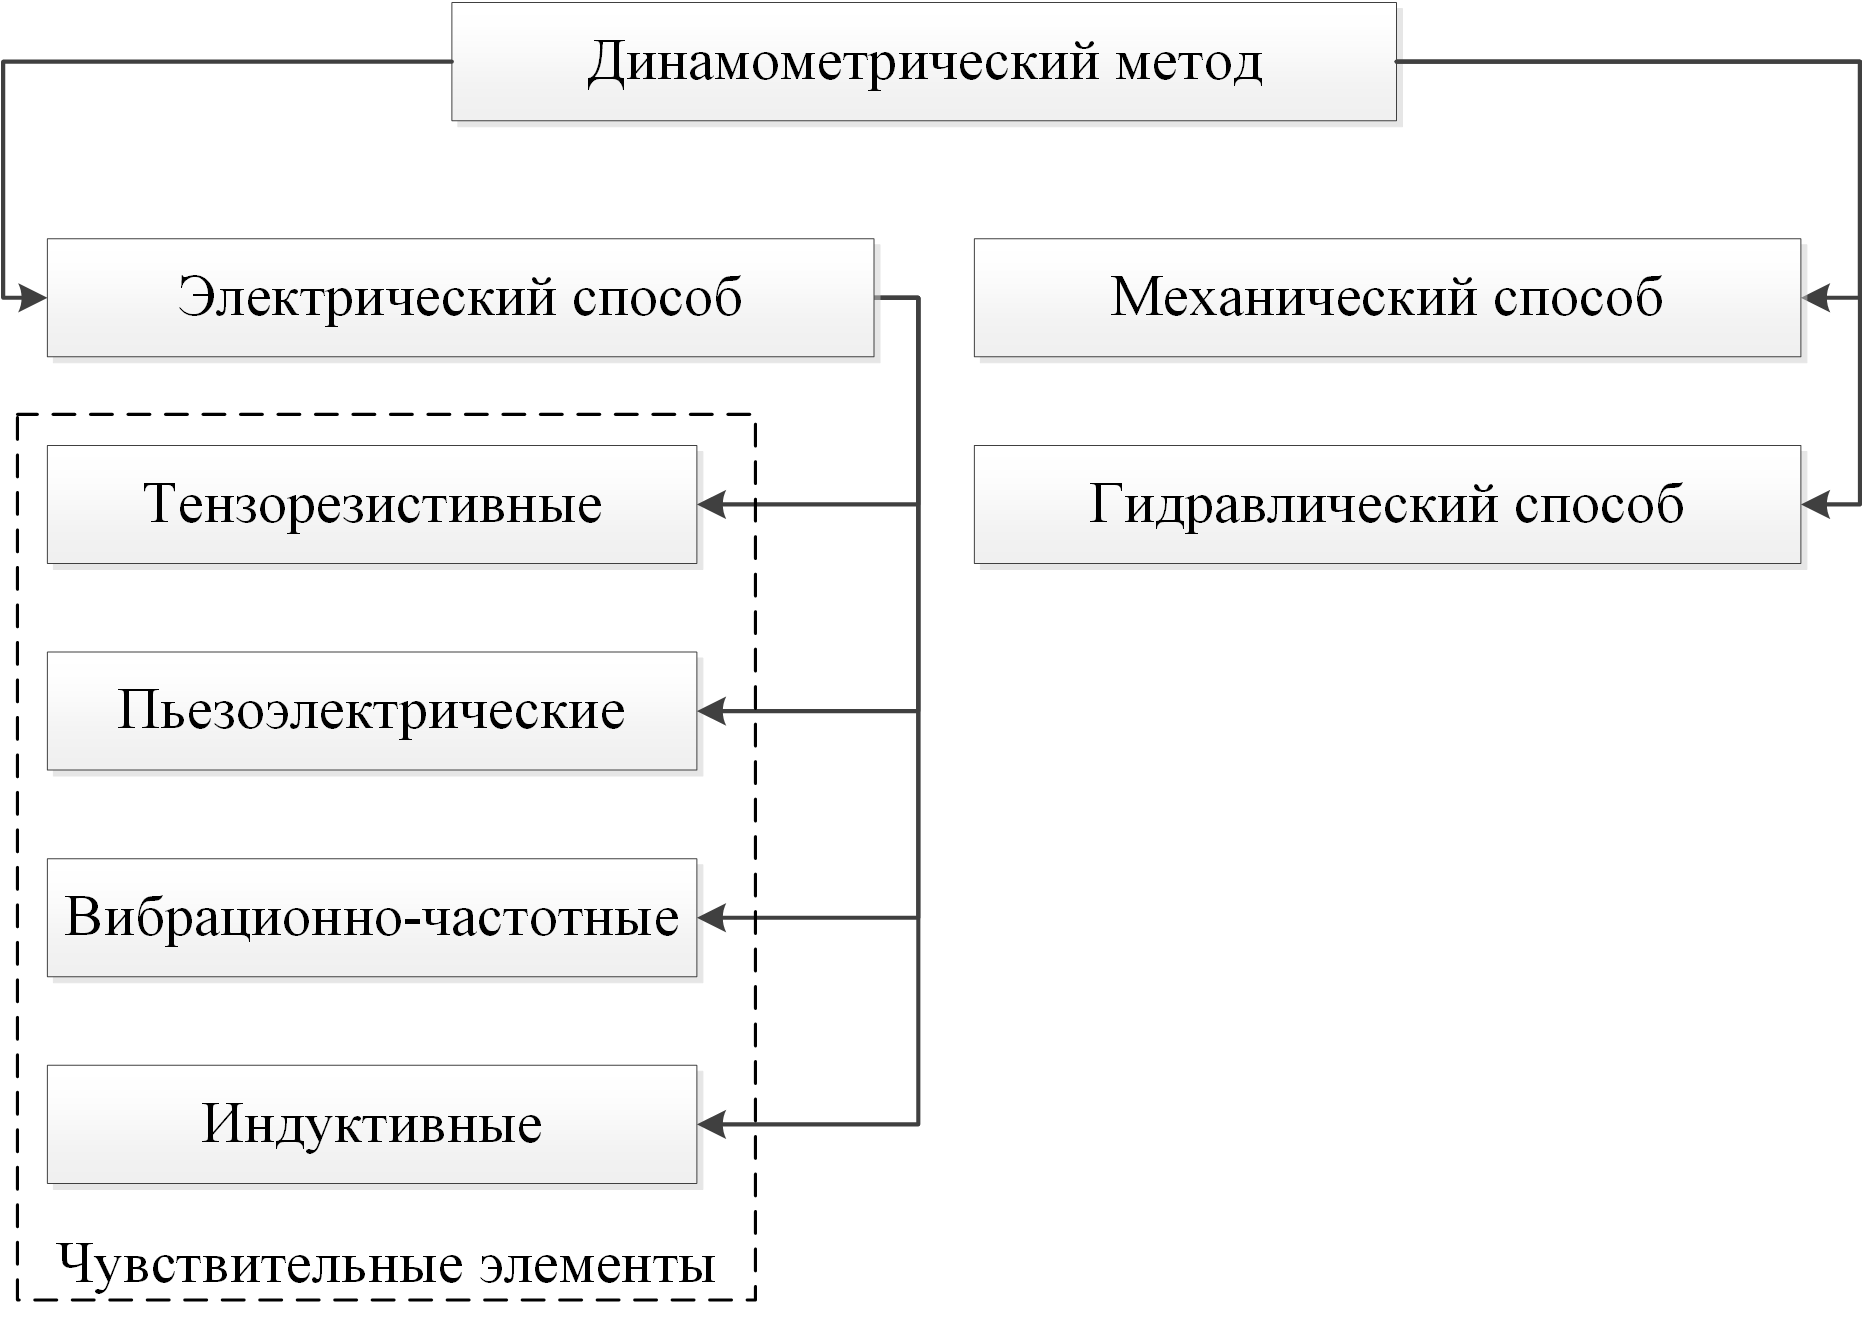
\includegraphics{MetodsControl}
	\caption{Методы контроля силовых параметров} 
	\label{img:MetodsControl}  
\end{figure}

Самым простым является механический способ так как представляет из себя прибор со шкалой либо автоматический самописец. Однако применение этого способа не целесообразно, так как имеются многочисленные недостатки, такие как: громоздкость чувствительного элемента, необходимость постоянной поверки и тарировки, не высокая точность из-за механического способа передачи информации, сложность считывания информации и т.д.

Гидравлический способ имеет в основном узко специализированное применение и не подходит для контроля силовых параметров рабочих органов из-за дороговизны и сложности конструкции.

Самым подходящим способом контроля является электрический. Он обеспечивает преобразование деформаций в электрический сигнал, который легко обрабатывать записывать и хранить. Так же одним из важнейших достоинств метода является малый размер чувствительных элементов, позволяющий устанавливать их в труднодоступных местах.

Электрический способ контроля силовых параметров обычно классифицирую в зависимости от используемых чувствительных элементов см. рисунок~\ref{img:MetodsControl}. Наиболее распространёнными являются тензорезистивные чувствительные элементы, так как:
\begin{itemize}
	\item обеспечивают достаточно высокую точность преобразования деформаций в электрический сигнал;
	\item наилучшим образом удовлетворяют критерию стоимость эффективность;
	\item могут использоваться при действии статических и динамических нагрузок;
	\item имеют линейную характеристику выходного сигнала \todo{[91]}.
\end{itemize}

\begin{table} [htbp]
	\centering
	%\captionsetup{width=17cm}
	\caption{Сравнение способов измерения усилия}
	\label{tbl:SposobIzm}
	\begin{tabular}{| l | c | c | c |}
		\hline
		\multirow{2}{*}{Критерии}&\multicolumn{3}{| c |}{Способы измерения} \\
		\cline{2-4}
		&Электрический&Механический&Гидравлический \\
		\hline
		\hline
		Стоимость				&$-$&$+$&$-$ \\
		Габаритные размеры		&$-$&$+$&$-$ \\
		Запись измерений		&$+$&$+$&$+$ \\
		Хранение измерений		&$+$&$-$&$-$ \\
		Обработка измерений		&$+$&$-$&$-$ \\
		Точность				&$+$&$-$&$+$ \\
		Сложность конструкции	&$+$&$-$&$-$ \\
		\hline
	\end{tabular}
\end{table}

\todo{Расписать то что представлено в таблицах}

\begin{table} [ht]%
	\centering
	\caption{Сравнение чувствительных элементов}%
	\label{tbl:SensItem}% label всегда желательно идти после caption
	\begin{SingleSpace}
		\setlength\extrarowheight{5pt} %вот этим управляем расстоянием между рядами, \arraystretch даёт неудачный результат
		\setlength{\tymin}{1.9cm}% минимальная ширина столбца
		\begin{tabulary}{\textwidth}{|>{\zz}L | >{\zz}C | >{\zz}C | >{\zz}C | >{\zz}C@{}|}
			\hline
			\multirow{2}{*}{Критерии}&\multicolumn{4}{ c |}{Чувствительные элементы} \\
			\cline{2-5}
			&Тензорезистивные&Пьезоэлектрические&Вибрационно-частотные&Индуктивные \\
			\hline
			\hline
			Точность преобразования	&$+$&$+$&$+$&$-$ \\
			Стоимость				&$+$&$-$&$-$&$-$ \\
			Динамические нагрузки	&$+$&$+$&$+$&$+$ \\
			Статические нагрузки	&$+$&$-$&$+$&$+$ \\
			Линейная характеристика	&$+$&$-$&$-$&$-$ \\
			Надёжность				&$+$&$-$&$-$&$-$ \\
			Доступность				&$+$&$-$&$-$&$+$ \\
			\hline
		\end{tabulary}%
	\end{SingleSpace}
\end{table}

\section{Основные выводы и задачи исследований}  \label{sect1_4}

Целью диссертационной работы является разработка метода контроля силы сопротивления прочных снежно-ледяных образований разрушению и обоснование параметров режима работы дискового режущего инструмента в зависимости от его износа.

Главными задачами проведенного комплекса научных исследований и технических разработок являются:
\begin{itemize}
	\item разработать комплекс средств контроля силы сопротивления прочных снежно-ледяных образований разрушению, возникающей в процессе взаимодействия дискового режущего инструмента с ними;
	\item исследовать влияние износа дискового режущего инструмента на силу сопротивления прочных снежно-ледяных образований разрушению;
	\item разработать математическую модель, позволяющую вычислить силу сопротивления прочных снежно-ледяных образований разрушению в зависимости от степени износа дискового режущего инструмента и шага резания;
	\item разработать метод контроля силы сопротивления прочных снежно-ледяных образований разрушению с целью минимизации энергоемкости процесса разрушения еще на стадии проектирования рабочих органов;
	\item разработать практические рекомендации по подбору радиуса закругления режущей кромки дискового режущего инструмента при проектировании рабочих органов спецмашин использующих такой инструмент.
\end{itemize}           % Глава 1
\chapter{Описание эксперимента}\label{chapt2}

Для модернизации существующих и создания новых рабочих органов предлагается использовать дисковый режущий инструмент, что позволяет снизить энергоёмкость и увеличить производительность. Основным контролируемым параметром, при оснащении рабочих органов уборочных машин дисковыми резцами, является сила сопротивления прочных СЛО резанию. Для более объективного изучения процесса взаимодействия дискового инструмента с прочными СЛО предлагается контролировать три составляющие силы резания: горизонтальную, боковую и вертикальную. Контроль составляющих непосредственно на рабочем органе требует больших трудозатрат, так как физические свойства (прочность, плотность, наличие абразивного материала) прочных СЛО на дорожных покрытиях постоянно меняются и зависят от: температуры окружающей среды, влажности, теплозапаса дорожного полотна и других фактором \todo{[ссылка]}, и дорогостоящего оборудования (датчики силы, оснастка для их монтажа). Опираясь на опыт работ по резанию мерзлых грунтов различными инструментами \todo{[ссылки]}, целесообразно исследовать в лабораторных условиях одиночный полноразмерный дисковый резец.

Целью проведения экспериментальных лабораторных исследований является выявления рационального радиуса закругления рабочей кромки дискового резца, а также оценки влияния шага резания, совместно с радиусом закругления рабочей кромки, на силовые показатели процесса разрушения прочных СЛО дисковым режущим инструментом.

\section{Условия проведения эксперимента}\label{sect2_1}

При проведении экспериментальных исследований использовались дисковые резцы с различным радиусом закругления рабочей кромки. Радиусы закругления составляли $R=[0,5\ 1,5\ 2,5\ 3,5\ 4,5]$ мм.
Остальные параметры приняты следующие: 
\begin{itemize}
	\item диаметр дискового резца $D=200$ мм.;
	\item величина заострения дискового резца $\delta=30^\circ$;
	\item глубина резания $h=60$ мм.;
	\item шаг резания $t=[10\ 20\ 30\ 40\ 50]$ мм.;
	\item задний угол $\gamma=3^\circ\div5^\circ$;
	\item температура окружающего воздуха $-$2~$\div\ -$7~${}^\circ$С;
	\item скорость резания $0,51\ \slantfrac{\text{м}}{\text{м}}$ ($1,84\ \slantfrac{\text{км}}{\text{ч}}$).
\end{itemize}
Применение таких параметров обуславливается раннее выполненными работами по данной тематике. \todo{добавить ссылок} На рисунке \ref{img:DirForse} приведено направление действия составляющих силы сопротивления резанию и способ установки дискового инструмента относительно разрушаемого массива.
\begin{figure} [htbp]
	\center
	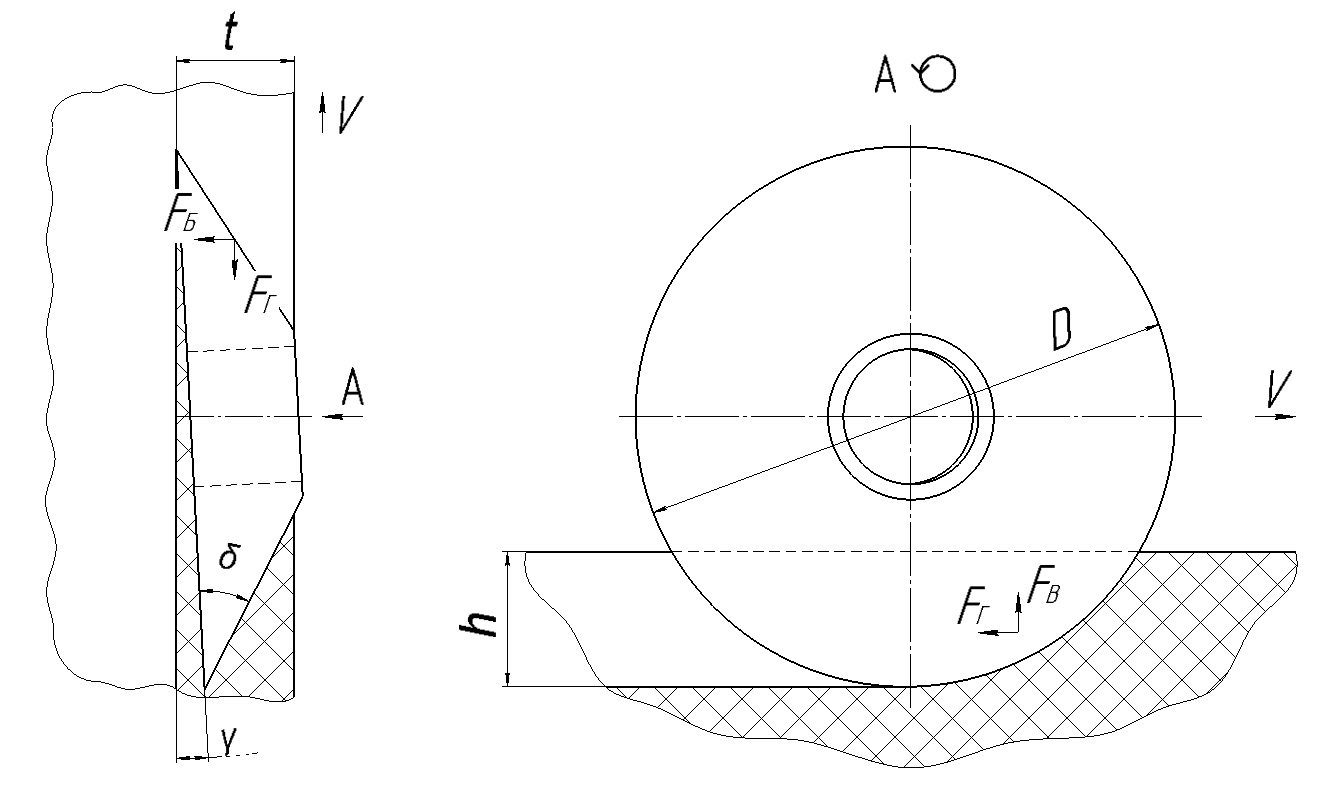
\includegraphics[width=1\textwidth]{DirForse}
	$t$ "--- шаг резания; $V$ "--- направление перемещения резца; $F_\text{Б}$ "--- боковая составляющая силы сопротивления резанию; $F_\text{Г}$ "--- горизонтальна составляющая силы сопротивления резанию; $D$ "--- диаметр дискового резца; $\delta$ "--- угол заострения дискового резца; $h$ "--- глубина резания; $F_\text{В}$ "--- вертикальная составляющая силы сопротивления резанию; $\gamma$ "--- угол установки дискового резца (задний угол). 
	\caption{Схема взаимодействия дискового резца с разрушаемым массивом} 
	\label{img:DirForse}  
\end{figure}

\section{Механизированный лабораторный стенд}\label{sect2_2}

\begin{figure} [htbp]
	\center
	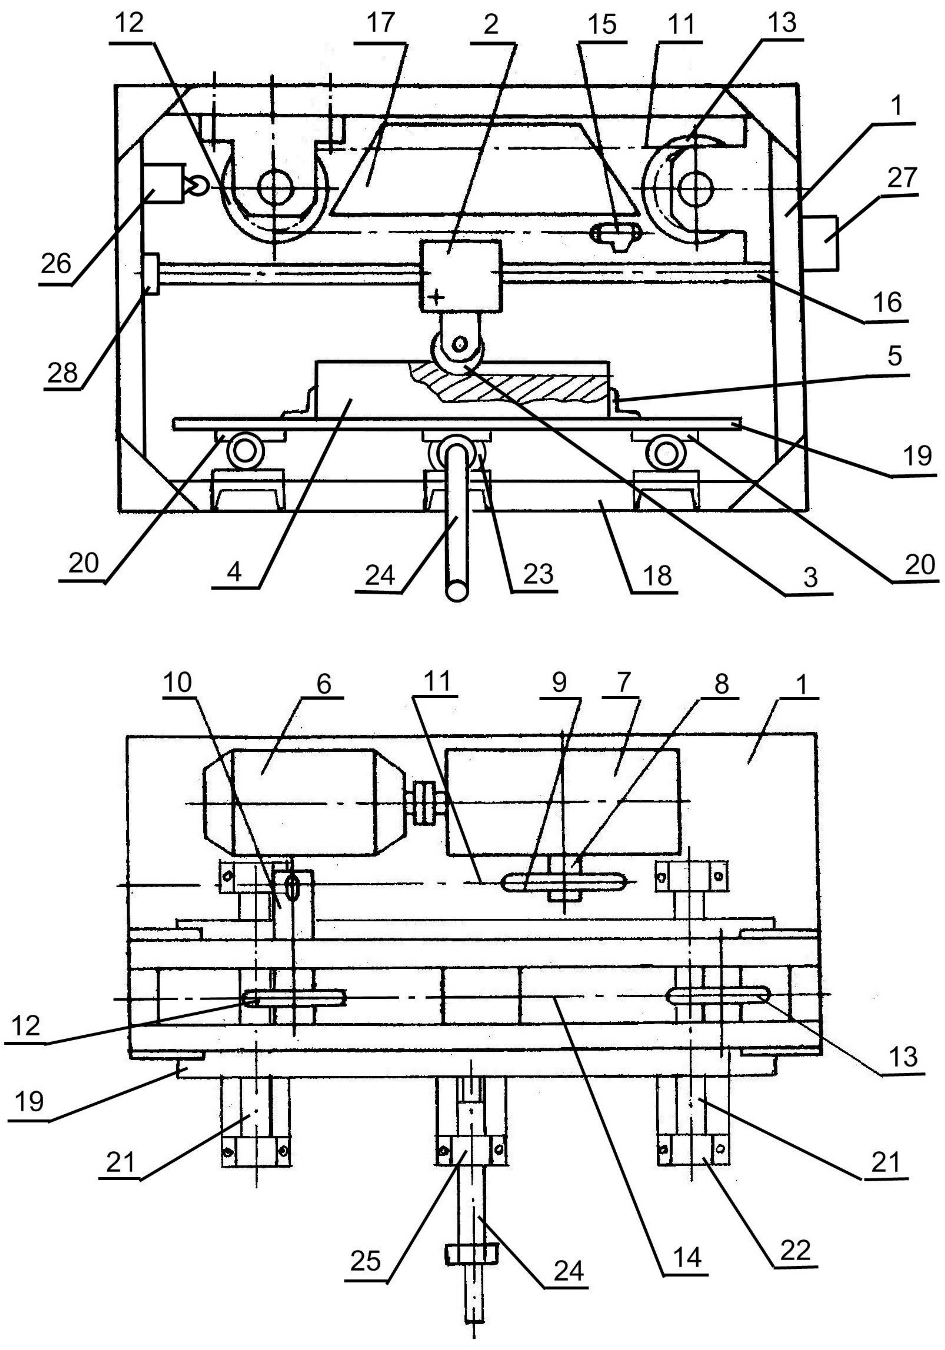
\includegraphics[scale=0.35]{Stend}
	
	1 "--- опорная рама; 2 "--- тензометрическая головка; 3 "--- режущий инструмент; 4 - образец льда; 5 "--- упоры; 6 "--- электрический двигатель; 7 "--- редуктор; 8 "--- выходной вал редуктора; 9 "--- приводная звездочка; 10 "--- ведущий вал цепной передачи; 11 "--- цепь; 12, 13 "--- звездочки тяговой цепи; 14 "--- тяговая цепь привода; 15 "--- захват; 16 "--- направляющие тензометрической головки; 17 "--- шина; 18 "--- нижняя балка рамы; 19 "--- несущая плита; 20 "--- подшипники скольжения; 21 "--- направляющие механизма поперечной подачи образца; 22 "--- опоры; 23 "--- ходовой механизм; 24 "--- поворотная рукоятка; 25 "--- опора поворотной рукоятки, 26 "--- конечный выключатель; 27 "--- кнопочная станция; 28 "--- демпферы.
	\caption{Схема лабораторного стенда} 
	\label{img:Stend}  
\end{figure}

Стенд содержит опорную раму 1 сварной конструкции, на которой смонтированы две цилиндрические направляющие 16, по которым перемещается тензометрическое звено 2 с закрепленным на нем режущим инструментом 3. На нижней балке 18 опорной рамы 1 стенда смонтирован механизм поперечной подачи образца 4 льда, включающий несущую плиту 19, к нижней поверхности которой, основанием вверх, прикреплены четыре подшипника скольжения 20, которые попарно сопряжены с двумя параллельными цилиндрическими направляющими 21, с возможностью продольного перемещения по ним. Концы направляющих 21 жестко закреплены в опорах 22, смонтированных на нижней балке 18 опорной рамы 1 стенда. В средней части несущей плиты 19, на ее нижней поверхности, установлен ходовой механизм 23, выполненный в виде втулки, на внутренней поверхности которой выполнена ходовая резьба.
 
С резьбой ходового механизма взаимодействует резьбовая часть поворотной рукоятки 24, цилиндрическая часть которой установлена в опоре 25 нижней части опорной рамы 1, с возможностью вращения в ней и без передвижения в осевом направлении. Образец льда 4 устанавливается на верхней поверхности несущей плиты 19 и жестко фиксируется упорами 5.

\begin{figure} [h]
	\center
	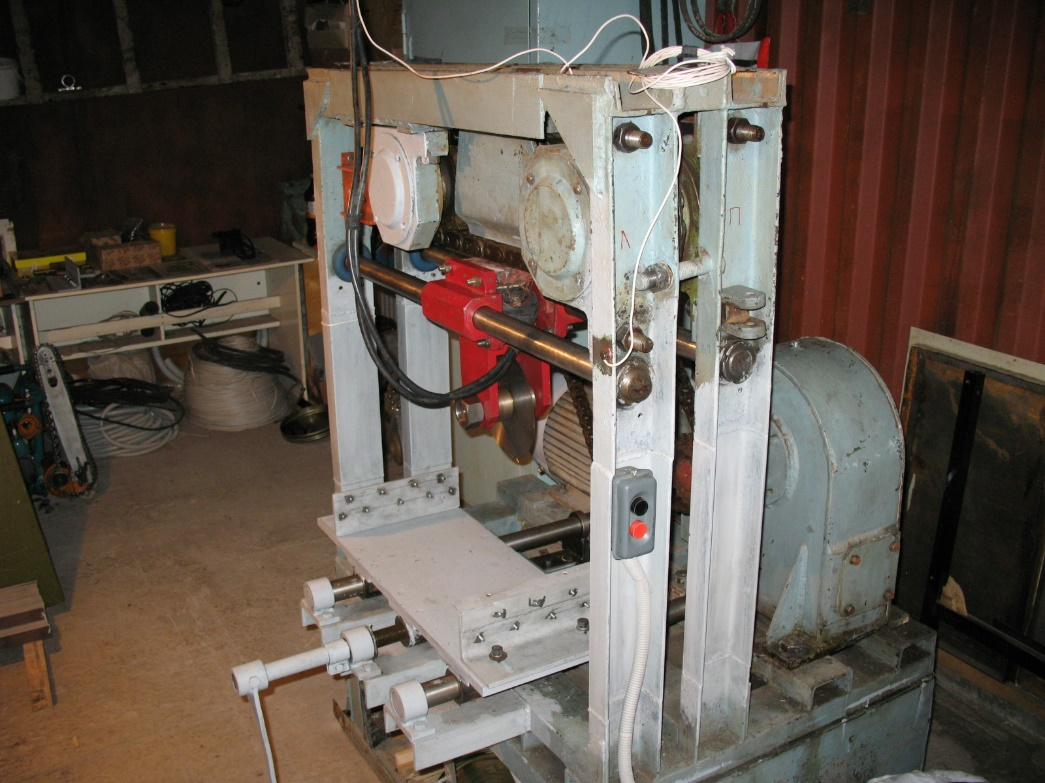
\includegraphics[width=\textwidth]{StendFoto}
	\caption{Внешний вид стенда для исследования процесса резания льда} 
	\label{img:StendFoto}  
\end{figure}

Привод тензометрической головки 2 включает электрический двигатель 6, червячный редуктор 7 с выходным валом 8, на котором закреплена звездочка 9 связанная со звездочкой ведущего вала 10 цепью 11, ведущую и ведомую звездочки 12, 13 тяговой цепи 14 привода. На одном из звеньев цепи 14 закреплен захват 15, при помощи которого, осуществляется перемещение тензометрической головки 2, по направляющим 16. Для предотвращения прогиба тяговой цепи 14 на опорной раме 1 установлена шина 17.

Управление электродвигателем 6 привода тензометрической головки 2 стенда осуществляется кнопочной станцией 27. Для автоматического отключения двигателя от электрической сети после проведения реза, на левой вертикальной опоре стенда установлен конечный выключатель 26. Окончательная остановка тензометрической головки в крайнем левом положении при резании на большой глубине, производится демпферами 28. Регулировка глубины резания, осуществляется с помощью калиброванных прокладок (на рисунках не показаны) и установкой режущего инструмента различной геометрической формы.

\section{Аппаратно-программный измерительный комплекс}\label{sect2_3}

Для контроля составляющих силы сопротивления прочных СЛО резанию необходимо спроектировать измерительный комплекс. Наиболее широкое распространение, для измерения различных сил резания, получил тензометрический метод контроля \todo{[ссылки]}. Он заключает в себе простоту и дешевизну измерений без потери точности измерений. Задача контроля силы сопротивления прочных СЛО резанию сводится к контролю электрического сопротивления чувствительных элементов.

\begin{figure} [htbp]
	\center
	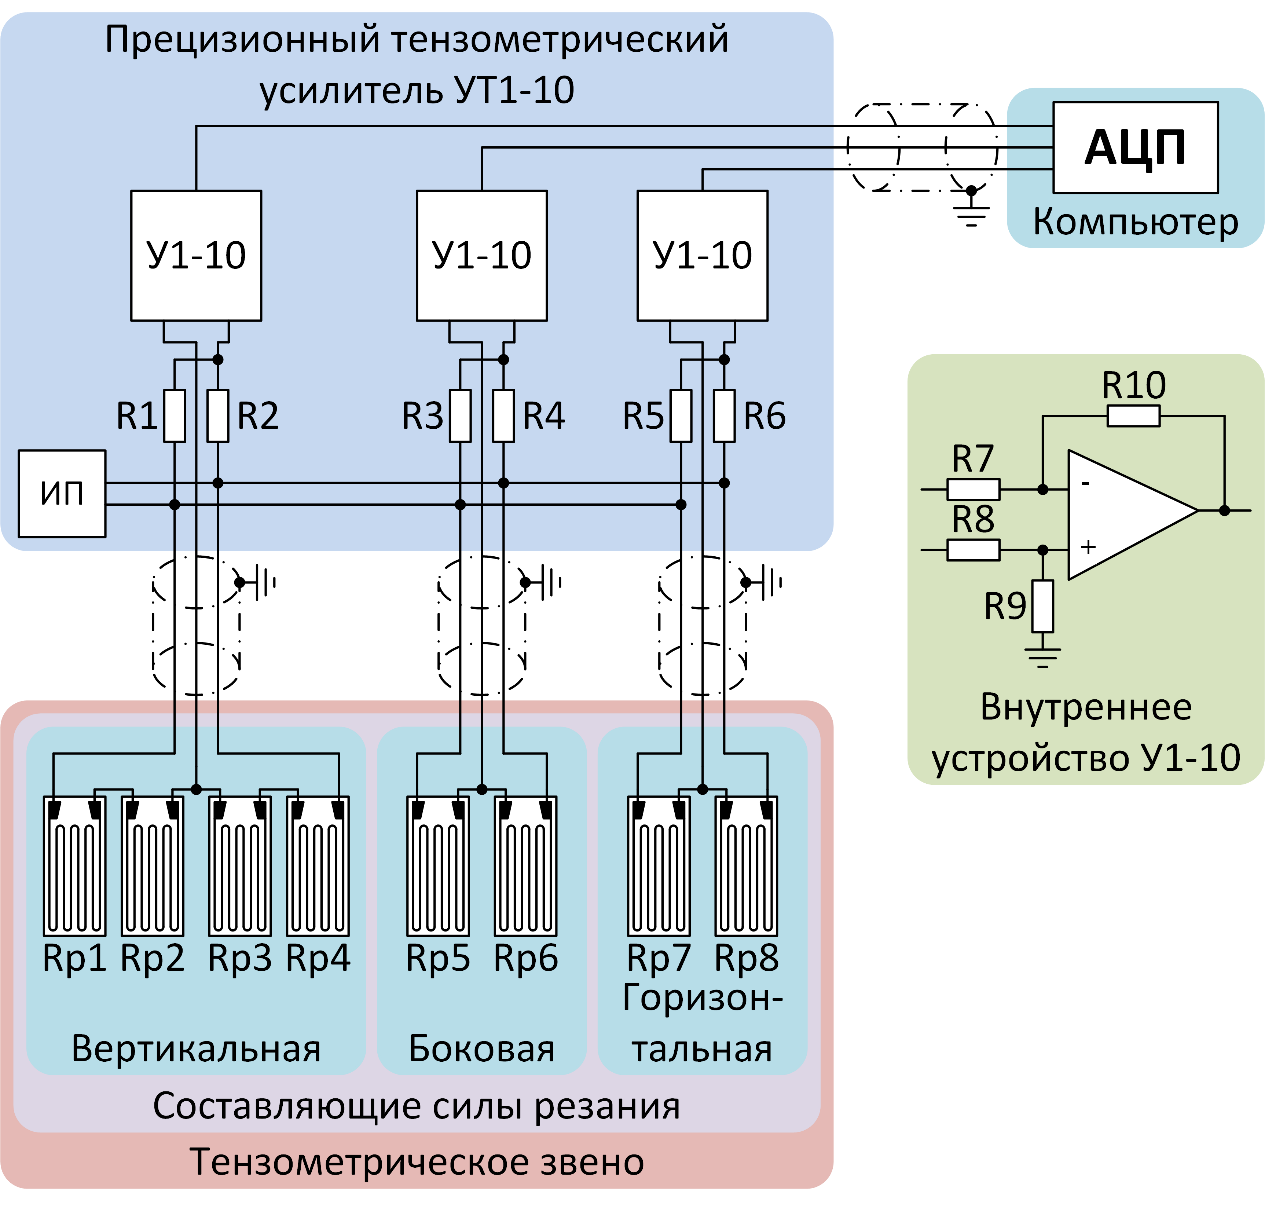
\includegraphics[width=\textwidth]{StructKomplex}
	\caption{Структурная схема измерительного комплекса для контроля силы сопротивления резанию} 
	\label{img:StructKomplex}  
\end{figure}

На рисунке \ref{img:StructKomplex} приведена структурная схема аппаратной составляющей измерительного комплекса, которая состоит из тензометрического звена, прецизионного тензометрического усилителя УТ1-10 и компьютера с установленной платой АЦП L-154. Все элементы комплекса соединены экранированным, заземлённым кабелем.

\subsection{Тензометрическое звено}\label{subsect2_3_1}

Чувствительным элементом комплекса является тензорезистор КФ5П1-20-200-А-12-С5. Имеющий следующие технические характеристики: 
\begin{itemize}
	\item номинальное электрическое сопротивление "--- $200$ Ом;
	\item ток питания "--- $20$ мА;
	\item диапазон измеряемых деформаций "--- $\pm3~000\cdot10^{-6}$;
	\item коэффициент тензочувствительности "--- $1,9\ldots2,3$ ;
	\item рабочая область температур "--- от $-$70 до $+$200~${}^\circ$С.
\end{itemize}

Тензорезистор наклеены на тензометрическое звено, представляющее собой круглую бобышку с тонкими стенками расположенную на прямоугольной плите, служащей для крепления его к лабораторному стенду. Изделие выполняется из стали марки 55С2. Такая конструкция обеспечивает наилучший уровень деформации тензорезисторов одновременно для всех составляющих силы сопротивления прочных СЛО резанию.

\begin{figure} [htbp]
	\center
	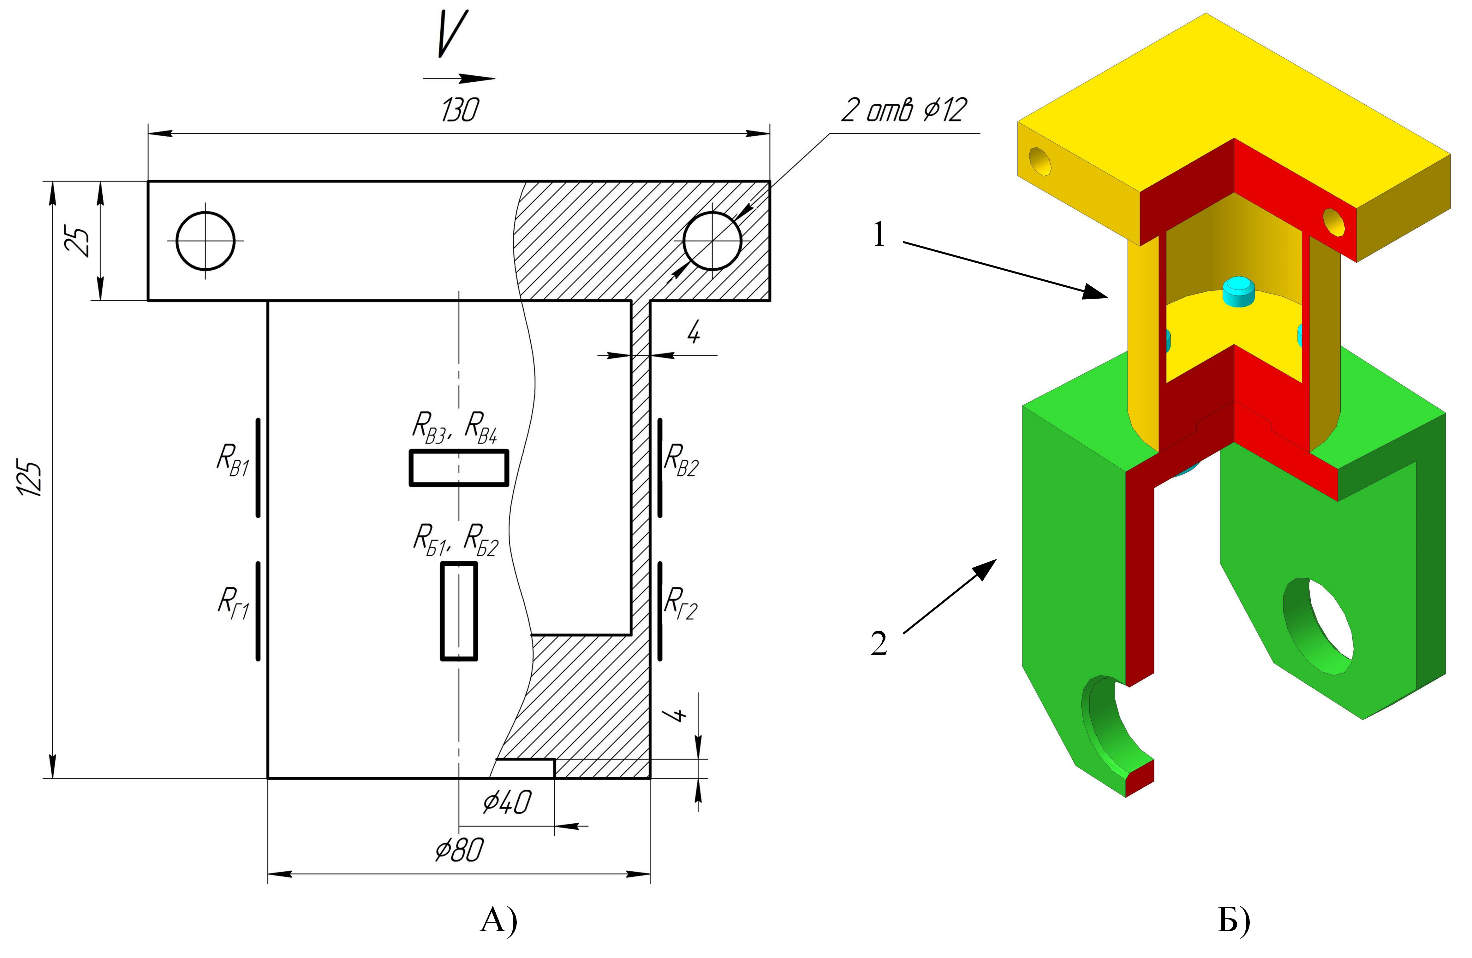
\includegraphics[width=\textwidth]{TenzoGolovka}
	
	А "--- схема наклейки тензорезисторов; Б "--- общий вид тензометрического звена;\\
	1 "--- тензометрическая головка; 2 "--- крепёж дискового режущего инструмента.
	\caption{Тензометрического звено} 
	\label{img:TenzoGolovka}  
\end{figure}

На рисунке \ref{img:TenzoGolovka} приведён общий вид тензометрического звена (Б) с установленным на него кронштейном (2) для крепления режущего инструмента. Тензометрической звено в сборе с дисковым инструментом устанавливается на лабораторный стенд описанный в \todo{[ссылки]}.

Также на рисунке \ref{img:TenzoGolovka} приведена схема наклейки тензорезисторов (А). Для измерения горизонтальной составляющей силы резания используется полу мостовая схема включения, с избирательной чувствительностью, тензорезистор $R_{\text{Г}1}$ включён в первое плечо измерительного моста, а $R_{\text{Г}2}$ – в четвёртое. Такая схема позволяет обеспечить избирательную чувствительность тензометрического моста к деформации изгиба (не чувствительна к деформации растяжения-сжатия), возникающей в следствии действия горизонтальной составляющей силы резания. Для боковой составляющей используется схема включения тензорезисторов аналогичная приведённой выше. Тензорезистор $R_{\text{Б}1}$ включён в первое плечо измерительного моста, а $R_{\text{Б}2}$ – в четвёртое. Для измерения вертикальной составляющей, диаметрально расположенные тензорезисторы $R_{\text{В}1}$ и $R_{\text{В}2}$ необходимо включить в одно плечо полумоста. Во второе плечо включаются компенсационные тензорезисторы $R_{\text{В}3}$ и $R_{\text{В}4}$, обеспечивающие также термокомпенсацию. Все схемы включения обеспечивают термокомпенсацию и компенсацию сопротивления соединительных проводов.


\subsection{Тензометрический усилитель}\label{subsect2_3_2}

Прецизионный тензометрический усилитель УТ1-10 имеет в основе прецизионный операционный усилитель (ОУ) 140УД17, двух полярный источник питания, калибровочные резисторы, стрелочные приборы указателя нулевого сигнала. ОУ имеет следующие характеристики:
\begin{itemize}
	\item максимальное выходное напряжение "--- $\pm12$ В;
	\item напряжение смещения нуля "--- $75$ мкВ;
	\item ток потребления "--- $4$ мА;
	\item коэффициент усиления напряжения – $200~000$;
	\item напряжение питания "--- $\pm(13,6\ldots16.5)$ В
	\item температура окружающей среды "--- $-$10$\ldots+$70~${}^\circ$С.;
\end{itemize}

Включение ОУ по дифференциальной схеме обеспечат исключительную чувствительность к изменению сопротивления, что в свою очередь повышает чувствительно всей системы к малому изменению нагрузки.


\subsection{Плата оцифровки сигнала}\label{subsect2_3_3}

Усиленный сигнал поступает на вход платы АЦП L-154, которая обеспечивает обработку и фиксацию сигнала в удобном для анализа виде. Плата АЦП имеет следующие характеристики:
\begin{itemize}
	\item разрядность "--- $12$ бит;
	\item диапазон входного сигнала "--- $\pm5,12$ В;
	\item максимальная частота преобразования "--- $70$ кГц;
	\item входное сопротивление "--- $2$ МОм;
\end{itemize}


\section{Тарировка тензозвена}\label{sect2_4}

Описать как проводилась тарировка, привести тарировочные графики

\section{Способ записи и хранения данных}\label{sect2_5}

Пояснить как и для чего записывать и хранить данные

\subsection{Съем данных с платы АЦП}\label{subsect2_5_1}

\subsection{Загрузка данных в MatLAB}\label{subsect2_5_2}

           % Глава 2
\chapter{Обработка эксперимента}

\section{Описание методов}
Описание методов регрессионного анализа очень кратко. Описание работы программного комплекса по работе с изображением, описание программного комплекса по работе с данными           % Глава 3
\chapter{Методика обоснования рационального радиуса рабочей кромки дискового инструмента} \label{chapt4}           % Глава 4
\chapter*{Заключение} \label{conclusion}						% Заголовок
\addcontentsline{toc}{chapter}{Заключение}	% Добавляем его в оглавление

%% Согласно ГОСТ Р 7.0.11-2011:
%% 5.3.3 В заключении диссертации излагают итоги выполненного исследования, рекомендации, перспективы дальнейшей разработки темы.
%% 9.2.3 В заключении автореферата диссертации излагают итоги данного исследования, рекомендации и перспективы дальнейшей разработки темы.
%% Поэтому имеет смысл сделать эту часть общей и загрузить из одного файла в автореферат и в диссертацию:


Основные результаты работы заключаются в следующем.
\input{common/concl}
И какая-нибудь заключающая фраза.
\begin{comment}
Последний параграф может включать благодарности.  В заключение автор
выражает благодарность и большую признательность научному руководителю
Иванову~И.И. за поддержку, помощь, обсуждение результатов и научное
руководство. Также автор благодарит Сидорова~А.А. и Петрова~Б.Б. за
помощь в работе с образцами, Рабиновича~В.В. за предоставленные
образцы и обсуждение результатов, Занудятину~Г.Г. и авторов шаблона
*Russian-Phd-LaTeX-Dissertation-Template* за помощь в оформлении
диссертации. Автор также благодарит много разных людей и
всех, кто сделал настоящую работу автора возможной.
\end{comment}      % Заключение
\chapter*{Список сокращений и условных обозначений}             % Заголовок
\addcontentsline{toc}{chapter}{Список сокращений и условных обозначений}  % Добавляем его в оглавление
\noindent
\addtocounter{table}{-1}% Нужно откатить на единицу счетчик номеров таблиц, так как следующая таблица сделана для удобства представления информации по ГОСТ
%\begin{longtabu} to \dimexpr \textwidth-5\tabcolsep {r X}
\begin{longtabu} to \textwidth {r X}
	\textbf{СЛО}	& снежно-ледяные образования\\
	\textbf{ПСЛО}	& прочные снежно-ледяные образования\\
	\textbf{СКО}	& среднеквадратичное отклонение (выборочное)
\end{longtabu}
        % Список сокращений и условных обозначений
%\include{Dissertation/dictionary}      % Словарь терминов
\include{Dissertation/references}      % Список литературы
%\include{Dissertation/lists}           % Списки таблиц и изображений (иллюстративный материал)
\input{Dissertation/appendixsetup}   % Предварительные настройки для правильного подключения Приложений
\chapter{Функции обработки данных эксперимента} \label{Appendix:FPE}

В данном приложении приведены все функции для предварительной обработки эксперементальных данных.

\section{Функция отброса грубых ошибок}\label{Appendix:FPE:DGE}

\noindent\textbf{Входные параметры:}
\begin{itemize}[leftmargin=1.25cm]
	\item [] \lstinline{y\_in} "--- массив измерененых значений (сигнал переходного процесса);
	\item [] \lstinline{f} "--- выбор режима работы: 1 "--- анализировать точки попавшие во вторую группу, 0 "--- анализировать только точки попавшие в третью группу.
\end{itemize}
\textbf{Выходные параметры:}
\begin{itemize}[leftmargin=1.25cm]
	\item [] \lstinline{out} "--- индексный массив с 0 и 1 указывающий индесы отбрасываемых точек.
\end{itemize}

\begin{lstlisting}[label={list:DropGrossError}]
	function out = DropGrossError(y_in, f)
		p_l = 5;    l=1;
		p_r = 0.1;  r=2;
		
		n = length(y_in);
		out = zeros(1, n);
		y_error = false(1, n);
		y_warn = false(1, n);
		y_good = false(1, n);
		y_idx = 1:n;
		e = true;
		while e
			y_idx_step = y_idx(~y_error);
			y_step = y_in(~y_error);
			
			n = length(y_step);
			t_tab = abs(...
				(tinv([p_l p_r] ./ 100, n - 2) .* sqrt(n-1)) ./ ...
				sqrt(n - 2 + tinv([p_l p_r] ./ 100, n - 2) .^ 2) ...
				);
			
			y_t = zeros(1, 2);
			ind_y_t = zeros(1, 2);
			
			[y_t(1), ind_y_t(1)] = max(y_step);
			[y_t(2), ind_y_t(2)] = min(y_step);
			
			[d_max, d_max_ind] = max(abs(y_t-mean(y_step)));    
			d_max_ind = ind_y_t(d_max_ind);
			
			t = d_max/std(y_step);
			
			e = t > t_tab(r);
			w = t_tab(l) < t & t < t_tab(r);
			g = t < t_tab(l);
			
			if w && f
				hFq = figure;
				plot(y_step);hold on
				plot(d_max_ind, y_step(d_max_ind), 'sr', ...
				'MarkerFaceColor','r')
				axis([0 n min(y_step)-2 max(y_step)+2])
				choice = ...
				    questdlg('Удалить отмеченну на графике точку?', ...
				             'Удаление грубых точек', ...
				             'Да','Нет','Нет');
				close(hFq)   
				e = strcmp('Да', choice);
			end
			
			y_error(y_idx_step(d_max_ind)) = e;
			y_warn(y_idx_step(d_max_ind)) = w;
			y_good(y_idx_step(d_max_ind)) = g;    
		end
		out(y_error) = 1;		
\end{lstlisting}        % Приложения

\end{document}
